\documentclass[11pt]{article}

\usepackage[a4paper,margin=2.5cm]{geometry}
\usepackage{amsmath}
\usepackage{amssymb}
\usepackage{graphicx}
\usepackage{booktabs}
\usepackage{listings}
\usepackage{placeins}
\usepackage{hyperref}

\graphicspath{{frontend/ops/dss/benchmark/}}
\lstset{basicstyle=\ttfamily\footnotesize,columns=fullflexible,
    keepspaces=true,breaklines=true,frame=single,showstringspaces=false}

\title{Cell-wise Storage, Batched Sum Factorization\\
and the Affine Laplacian in SFEM}
\author{}
\date{\today}

\begin{document}
\maketitle

\section{Introduction}

The direction of this work is inspired by the main idea behind
\texttt{FlexibleCG.pdf}: reduce the cost of repeated matrix-free operator
applications by changing the data layout used by the high-order element kernels.
Instead of applying the operator directly from a unique global vector at every
iteration, we introduce a persistent cell-wise representation.

In the standard finite element representation, each global degree of freedom is
stored once. Adjacent elements refer to the same global value through an
element-local to global map. This representation is compact and natural for
assembled algebra, but a matrix-free tensor-product kernel sees indirect memory
accesses every time it gathers element data.

The cell-wise representation duplicates shared degrees of freedom per element.
Each element owns a dense local tensor of values. This increases memory usage,
but makes the data consumed by the volume kernel regular, contiguous, and
amenable to blocking and vectorization. After an element-wise operator
application, duplicated values must be synchronized by a direct stiffness
summation (DSS) step. This note documents the conversion from the global SFEM
vector representation to the blocked cell-wise layout BXYZE, the batched
sum-factorization kernel for reference gradients, and the complete affine
Laplacian that combines gradients, metric application and transpose evaluation.
Component and complete-operator benchmarks are reported separately.

\section{Memory Layout: Global to BXYZE}

\subsection{SFEM semi-structured connectivity}

For a semi-structured hexahedral mesh of level \(p\), each macro element has
\[
    N = p + 1
\]
nodes per coordinate direction and therefore
\[
    n_{\mathrm{loc}} = N^3
\]
local scalar degrees of freedom.

SFEM stores the element connectivity in structure-of-arrays form:
\[
    \mathrm{elements}[\ell][e] = g.
\]
Here \(e\) is the element index, \(\ell\) is the local node index, and \(g\) is
the corresponding global node id. For tensor-product hexahedra we use the local
ordering
\[
    \ell(i_x,i_y,i_z) = i_z N^2 + i_y N + i_x,
\]
with
\[
    0 \le i_x,i_y,i_z < N.
\]
Thus \(i_x\) is the fastest local coordinate.

The global scalar vector is denoted by
\[
    u_g[g].
\]
The goal of the conversion is to construct a cell-wise vector \(u_c\) such that
each element-local copy satisfies
\[
    u_c(e,i_x,i_y,i_z) =
    u_g\left[\mathrm{elements}[\ell(i_x,i_y,i_z)][e]\right].
\]

\subsection{Element blocks}

The BXYZE layout groups elements into fixed-size blocks of \(B\) elements. This
\(B\) is a data-layout block size, not an SFEM mesh block. For an element \(e\),
we define
\[
    e_b = \left\lfloor \frac{e}{B} \right\rfloor,
    \qquad
    b = e \bmod B.
\]
The index \(e_b\) identifies the element block, while \(b\) identifies the lane
inside that block.

For example, if \(B=4\), then
\[
\begin{array}{c|cccccc}
e   & 0 & 1 & 2 & 3 & 4 & 5 \\
\hline
e_b & 0 & 0 & 0 & 0 & 1 & 1 \\
b   & 0 & 1 & 2 & 3 & 0 & 1
\end{array}
\]
The last block may be partially filled. Missing lanes are padding lanes and are
set to zero by the conversion.

\subsection{BXYZE linearization}

The BXYZE linear index used in the current SFEM prototype is
\[
    I(e_b,i_z,i_y,i_x,b)
    =
    b
    + B\left(
        i_x
        + N\left(
            i_y
            + N\left(
                i_z + N e_b
            \right)
        \right)
    \right).
\]
Equivalently, the strides are
\[
\begin{array}{c|c}
\text{index} & \text{stride} \\
\hline
b   & 1 \\
i_x & B \\
i_y & BN \\
i_z & BN^2 \\
e_b & BN^3
\end{array}
\]
Thus, for fixed \((e_b,i_x,i_y,i_z)\), the \(B\) element lanes are contiguous in
memory:
\[
    u_c[I + 0],\ u_c[I + 1],\ \ldots,\ u_c[I + B-1].
\]
This is the key property of the layout. The volume kernel can operate on the
same local tensor point across several elements with contiguous memory accesses
in the element-lane dimension.

\subsection{Conversion algorithm}

Let
\[
    n_{\mathrm{blocks}} =
    \left\lceil \frac{n_{\mathrm{elements}}}{B} \right\rceil .
\]
The allocated number of scalar values is
\[
    n_{\mathrm{values}} = n_{\mathrm{blocks}}\,B\,N^3.
\]

The conversion iterates over element blocks and local tensor coordinates:
\[
\begin{aligned}
\text{for } e_b &= 0,\ldots,n_{\mathrm{blocks}}-1,\\
\text{for } i_z,i_y,i_x &= 0,\ldots,N-1.
\end{aligned}
\]
For the current block,
\[
    e_{\mathrm{begin}} = e_b B,
    \qquad
    r = n_{\mathrm{elements}} - e_{\mathrm{begin}},
\]
and the number of valid lanes is
\[
    b_{\mathrm{count}} = \min(r,B).
\]
Then, for each valid lane \(b < b_{\mathrm{count}}\), the element index is
\[
    e = e_{\mathrm{begin}} + b,
\]
and the conversion performs
\[
    u_c[I(e_b,i_z,i_y,i_x,b)]
    =
    u_g\left[
        \mathrm{elements}[\ell(i_x,i_y,i_z)][e]
    \right].
\]
For padded lanes \(b_{\mathrm{count}} \le b < B\), the output is set to zero.

In code, the inner access pattern is intentionally simple:
\[
    \mathrm{gid} = \mathrm{elements}[\ell][e_{\mathrm{begin}} + b],
    \qquad
    \mathrm{dst}[b] = u_g[\mathrm{gid}].
\]
Since SFEM stores \(\mathrm{elements}[\ell][e]\) contiguously in \(e\), the
connectivity row is read contiguously over \(b\). The output \(\mathrm{dst}[b]\)
is also contiguous over \(b\). The only remaining indirect access is the read
from the global vector \(u_g[\mathrm{gid}]\), which is paid once when building
the persistent cell-wise representation.

\subsection{Current implementation scope}

The current implementation is scalar-field, CPU-side, and targets
semi-structured hexahedral meshes with explicit \(p\)-level tensor-product
indexing. The public conversion entry points are implemented in
\path{operators/dss/sfem_dss_bxyze.cpp} and declared in
\path{operators/dss/sfem_dss_bxyze.hpp}. The current code provides
single-precision and double-precision variants:
\[
    \texttt{sfem\_dss\_global\_to\_bxyze\_real32},
    \qquad
    \texttt{sfem\_dss\_global\_to\_bxyze\_real64}.
\]

The following section describes how the volume computation consumes this
storage. The gradient benchmark is a component benchmark: integration and DSS
are outside the operations measured here.

\section{Batched Sum Factorization for Reference Gradients}
\label{sec:sum-factorization}

\subsection{Problem and purpose of sum factorization}

On one reference hexahedron, the scalar finite element field is
\[
 \widehat u(\xi,\eta,\zeta)
 = \sum_{i,j,k=0}^{N-1}
   u_{ijk}\,\ell_i(\xi)\ell_j(\eta)\ell_k(\zeta),
 \qquad N=p+1.
\]
The input contains \(N^3\) nodal coefficients. The immediate goal is to compute
the three reference derivatives at a tensor grid of \(Q^3\) quadrature points.
These are intermediate quantities for a matrix-free Laplacian: geometry,
quadrature weights, transpose contractions and DSS follow later.

The setup constructs the one-dimensional matrices
\[
 S_{qi}=\ell_i(\xi_q), \qquad D_{qi}=\ell_i'(\xi_q),
 \qquad S,D\in\mathbb R^{Q\times N}.
\]
Applying \(S\) interpolates along one coordinate; applying \(D\) evaluates a
derivative along that coordinate. The three gradients require
\[
\begin{array}{c|ccc}
 & x\text{ direction} & y\text{ direction} & z\text{ direction}\\
\hline
 g_x & D & S & S\\
 g_y & S & D & S\\
 g_z & S & S & D
\end{array}
\]
where \(x,y,z\) denote reference-coordinate directions in this section.

A direct evaluation would combine all \(N^3\) coefficients separately at each
of the \(Q^3\) points, costing order \(N^3Q^3\) operations per component.
Sum factorization exploits the product structure of the basis: it transforms
one coordinate at a time, storing partial results between directions. One
component then involves
\[
 N^3Q + N^2Q^2 + NQ^3
\]
scalar multiplication terms per component. With
\(Q=N\), the scaling changes from order \(N^6\) to order \(N^4\).
Both the nine- and eight-contraction versions below already use sum
factorization; their difference is the reuse between gradient components.

\subsection{Classical element-wise evaluation: nine contractions}

The original reference gathers one element from the unique global vector and
evaluates its gradient components independently:
\begin{lstlisting}[language=C++]
for (ptrdiff_t e = 0; e < nelements; ++e) {
    for (int v = 0; v < N*N*N; ++v)
        element_u[v] = x_global[elements[v][e]];

    triad(D, S, S, element_u, gx_e);
    triad(S, D, S, element_u, gy_e);
    triad(S, S, D, element_u, gz_e);
}
\end{lstlisting}
The actual SFEM routine is \texttt{lagrange\_hex\_triad\_interpolate}, in
\path{operators/spectral_hex/lagrange_hex_laplacian_inline.hpp}.
For matrices \(B_0,B_1,B_2\), one call executes the following three loop nests.
Multidimensional notation denotes flattened arrays. For readability the sums
start at zero here; the implementation initializes from the first product.

\noindent\begin{minipage}{\linewidth}
\begin{lstlisting}[language=C++]
// x contraction: [k][j][i] -> [qx][k][j]
for (int qx = 0; qx < Q; ++qx)
    for (int k = 0; k < N; ++k)
        for (int j = 0; j < N; ++j) {
            scalar_t acc = 0;
            for (int i = 0; i < N; ++i)
                acc += B0[qx][i] * u[k][j][i];
            T1[qx][k][j] = acc;
        }
\end{lstlisting}
\end{minipage}
\par\medskip

\noindent\begin{minipage}{\linewidth}
\begin{lstlisting}[language=C++]
// y contraction: [qx][k][j] -> [qy][qx][k]
for (int qy = 0; qy < Q; ++qy)
    for (int qx = 0; qx < Q; ++qx)
        for (int k = 0; k < N; ++k) {
            scalar_t acc = 0;
            for (int j = 0; j < N; ++j)
                acc += B1[qy][j] * T1[qx][k][j];
            T2[qy][qx][k] = acc;
        }
\end{lstlisting}
\end{minipage}
\par\medskip

\noindent\begin{minipage}{\linewidth}
\begin{lstlisting}[language=C++]
// z contraction: [qy][qx][k] -> [qz][qy][qx]
for (int qz = 0; qz < Q; ++qz)
    for (int qy = 0; qy < Q; ++qy)
        for (int qx = 0; qx < Q; ++qx) {
            scalar_t acc = 0;
            for (int k = 0; k < N; ++k)
                acc += B2[qz][k] * T2[qy][qx][k];
            out[qz][qy][qx] = acc;
        }
\end{lstlisting}
\end{minipage}

After the first phase, only x is at quadrature points; after the second, x and y
are at quadrature points; after the third, all coordinates are. The temporary
orderings make the reduction index contiguous in each phase. The three calls
use \((B_0,B_1,B_2)=(D,S,S),(S,D,S),(S,S,D)\), respectively.
Each performs three directional contractions, giving \(3+3+3=9\) in total.
A contraction here means one complete directional transform, not one inner
dot product.

\subsection{Joint evaluation: eight contractions}

The paths for \(g_y\) and \(g_z\) both start by computing \(S_xu\).
Independent calls compute that same intermediate twice. Joint evaluation
retains it and branches afterwards:
\[
\begin{aligned}
 \text{x phase:}\quad & s_x=S_xu, & d_x&=D_xu,\\
 \text{y phase:}\quad & A_x=S_yd_x, & A_y&=D_ys_x, & A_z&=S_ys_x,\\
 \text{z phase:}\quad & g_x=S_zA_x, & g_y&=S_zA_y, & g_z&=D_zA_z.
\end{aligned}
\]
This requires \(2+3+3=8\) directional contractions. It evaluates the same
mathematical derivatives and does not change the basis, quadrature or geometry.
It applies on tensor-product hexahedra independently of whether their mapping
is affine; geometry is applied to the reference gradients afterwards.

The multiplication-term counts for the two schedules are
\[
\begin{aligned}
 C_9 &= 3N^3Q+3N^2Q^2+3NQ^3,\\
 C_8 &= 2N^3Q+3N^2Q^2+3NQ^3.
\end{aligned}
\]
For \(Q=N\), these become \(9N^4\) and \(8N^4\): one ninth of the
products is removed. This is not a prediction of an identical reduction in
wall time. The implementation also shares input loads when forming \(s_x,d_x\)
and fuses the three y and z paths, changing memory traffic and compiler behavior.

The implementation is
\texttt{sfem\_dss\_bxyze\_lagrange\_gradient} in
\path{operators/dss/sfem_dss_bxyze_affine_laplacian_inline.hpp}.
The reuse itself is independent of batching: the same routine with
\texttt{B\_EXEC=1} and input stride 1 provides an element-wise reference with
eight contractions.

\subsection{Storage blocks and execution batches}

We distinguish two parameters:
\[
 B_s=B_{\mathrm{save}}=\texttt{element\_block\_size},\qquad
 B_e=B_{\mathrm{exec}}=\texttt{execution\_block\_size}.
\]
The \(B\) used in the preceding storage section is \(B_s\). It controls
the persistent input layout and its nodal stride. The execution batch size
\(B_e\) controls how many elements are processed by one gradient-kernel call.
For now, \(B_e\leq B_s\) and \(B_s\bmod B_e=0\).

Storage block \(e_b\) contains \(B_s/B_e\) execution batches. For batch
\(t\) inside the block, the first input pointer is
\[
 u_0=u_c+e_bN^3B_s+tB_e.
\]
The nodal value for batch lane \(b\) is accessed as
\[
 u_0\left[(kN^2+jN+i)B_s+b\right],\qquad 0\leq b<B_e.
\]
Thus the same node across the batch is contiguous, even when \(B_e<B_s\).
The contraction loops reduce over the nodal coordinate and update all batch
lanes in their innermost loop:
\begin{lstlisting}[language=C++]
for (int i = 1; i < N; ++i) {
    const scalar_t s = S[qx*N + i];
    const scalar_t d = D[qx*N + i];
    const real_t *src = input + i*B_save;
    #pragma omp simd
    for (int b = 0; b < B_EXEC; ++b) {
        sum_s[b] += s * src[b];
        sum_d[b] += d * src[b];
    }
}
\end{lstlisting}
Different lanes belong to different elements, so no reduction between lanes is
needed. Each matrix coefficient is shared across the lanes. The template
parameters \(N,Q,B_e\) give the compiler fixed loop bounds; \(B_s\) remains
the input stride. The removed runtime \texttt{lane\_count} argument is not
needed for a full batch.
An earlier version still used that runtime count as the lane-loop bound even
though \(B_e\) was a template parameter. Diagnostic runs showed a substantial
timing penalty. All measurements reported here use the fixed
\texttt{b < B\_EXEC} loops; padding or full-block preconditions keep that bound
valid without a per-lane tail test.

OpenMP distributes storage blocks between threads with a static schedule.
Each thread processes the batches of its blocks sequentially and owns one
scratch slice. Thread count and batch size are independent: eight threads with
\(B_e=8\) means that each thread processes batches of eight elements, not
that one batch is split between eight threads.

The final gradient layout is
\[
 [\text{component}][\text{batch}][q_z][q_y][q_x][b].
\]
Its innermost stride uses \(B_e\), whereas the persistent input uses \(B_s\).
These gradient buffers are auxiliary quadrature data, not the final nodal
Laplacian vector in the persistent storage layout.

\subsection{Full batches, padding and current scope}

Padding makes fixed bounds possible without testing the number of valid
elements inside each contraction loop. A storage allocation can hold
\[
 n_{\mathrm{stored}}=
 B_s\left\lceil\frac{n_{\mathrm{elements}}}{B_s}\right\rceil
\]
elements, with the missing lanes of the final storage block filled with zero
by the existing global-to-BXYZE conversion. If \(B_s\) is divisible by
\(B_e\), every batch then has \(B_e\) allocated lanes. Applying this linear
gradient kernel to a zero padding lane gives zero gradients. Its output
allocation must also include the padding, and only real elements contribute to
validation, reductions or later global assembly. Connectivity and geometry for
nonexistent elements must not be read or constructed as if they were real cells.

\emph{The current benchmark deliberately tests full blocks:}
\[
 n_{\mathrm{elements}}\bmod B_s=0,\qquad B_s\bmod B_e=0.
\]
It rejects incompatible configurations before writing the CSV. Therefore the
measured kernel has fixed \(B_e\)-length loops, and the reported timings do
not include an execution tail or the cost of computing dummy elements. The
conversion already supports zero padding; extending the driver to execute
padded tail batches and to exclude them downstream remains separate work.

There is also padding between per-thread scratch slices, described below.
That padding separates memory regions and is unrelated to dummy element lanes.

\subsection{Workspace size, partition and lifetime}

The explicit workspace consists of two x-stage buffers and three buffers for
one y-quadrature slice:
\begin{center}
\begin{tabular}{lll}
\toprule
Buffers & Logical shape & Total scalar values\\
\midrule
\texttt{sx}, \texttt{dx} & $[i_z][i_y][q_x][b]$ & $2N^2QB_e$\\
\texttt{sy\_dx}, \texttt{dy\_sx}, \texttt{sy\_sx}
 & $[i_z][q_x][b]$ & $3NQB_e$\\
\bottomrule
\end{tabular}
\end{center}
The outer y-quadrature loop constructs these three slice buffers for one
\(q_y\), completes every z contraction for that slice, and then reuses their
storage for the next \(q_y\). Consequently they need \(3NQB_e\) values,
rather than \(3NQ^2B_e\).

Define \(C_x=N^2QB_e\) and \(C_y=NQB_e\). The five starting offsets are
\[
\begin{array}{c|ccccc}
\text{buffer} & \texttt{sx} & \texttt{dx} & \texttt{sy\_dx}
 & \texttt{dy\_sx} & \texttt{sy\_sx}\\
\hline
\text{offset} & 0 & C_x & 2C_x & 2C_x+C_y & 2C_x+2C_y
\end{array}
\]
so the workspace query returns
\[
 W=2C_x+3C_y=(2N^2Q+3NQ)B_e
\]
values of type \texttt{scalar\_t}, not bytes. The query and allocation happen
before timing:
\begin{lstlisting}[language=C++]
constexpr ptrdiff_t W =
    sfem_dss_bxyze_lagrange_gradient_workspace_n_values<N, Q, BE>();
constexpr ptrdiff_t gap = 128 / sizeof(scalar_t);
constexpr ptrdiff_t stride = ((W + gap - 1) / gap + 1) * gap;

std::vector<scalar_t> storage((size_t)nthreads * stride);
std::vector<scalar_t *> workspace_by_thread(nthreads);
for (int t = 0; t < nthreads; ++t)
    workspace_by_thread[t] = storage.data() + t * stride;
\end{lstlisting}
The extra gap follows the benchmark's per-thread separation strategy; it does
not change the useful workspace size \(W\) or promise that the allocation base
has a particular alignment. Each thread reuses its pointer for every batch it
owns. The kernel partitions the supplied slice internally, performs no heap
allocation and writes every intermediate before reading it. No workspace reset
is required between calls. The total scratch allocation scales with the number
of concurrent threads, not the number of mesh elements.

For \(p=8\), \(N=Q=9\), \(B_e=8\), the explicit scratch is
\(W=13608\) scalars, or \(106.3125\) KiB in double precision per thread
before the separation gap. At \(B_e=16\), it doubles to \(212.625\) KiB.
Small local accumulators are internal to the kernel; the three output buffers
are excluded from \(W\). A batch's gradients require another \(3Q^3B_e\)
scalars. They could be consumed by subsequent Laplacian stages and then reused;
the current benchmark instead retains the gradients of every element.

\subsection{Three-way benchmark and measurement boundaries}

The driver is
\path{frontend/ops/dss/benchmark/sfem_DSSBXYZEGradientBench.cpp}.
It compares three paths on the same random global field:
\begin{enumerate}
 \item \textbf{Global 9:} gather one element into a contiguous buffer, then call
 the original three independent SFEM tensor evaluations.
 \item \textbf{Global 8:} perform the same gather, then call the joint gradient
 kernel with \(B_e=1\) and input stride 1. Its input remains a unique global
 vector; the contiguous element buffer is temporary.
 \item \textbf{Cell-wise 8:} read the persistent BXYZE input and call the same
 joint gradient kernel on \(B_e\) elements at a time.
\end{enumerate}
The first comparison captures the changes associated with joint evaluation;
the second compares the two eight-contraction paths, including layout,
batching, gather elimination and their different memory access patterns.
Changing from nine to eight also changes fusion and intermediate ordering, so
the measured gain is not solely the arithmetic saving of one contraction.

Every timed apply reads \(S,D\) and the field, reads and writes intermediates,
and writes all three gradients for the entire mesh. Both global paths include
their connectivity reads and gather writes. Output stores and OpenMP region
entry/exit and synchronization are included. Mesh creation, quadrature and basis
setup, conversion, allocations, workspace pointer setup, correctness checks and
CSV writes are excluded. There is no metric multiplication, quadrature-weight
application, transpose contraction, scatter or DSS in these timings.

The output allocations have the following shapes:
\[
\begin{aligned}
 \text{Global 9 and Global 8:}&\quad
 [\text{component}][e][q_z][q_y][q_x],\\
 \text{Cell-wise 8:}&\quad
 [\text{component}][\text{batch}][q_z][q_y][q_x][b].
\end{aligned}
\]
They contain the same \(3n_{\mathrm{elements}}Q^3\) scalars for full batches.
They are separate allocations for the three methods and are overwritten on
each apply. Stores target process memory through the CPU caches; these timings
are not direct measurements of DRAM bandwidth.

The recorded sweep uses Apple M4 Pro code generation, double-precision input
and arithmetic, \(p\in\{2,4,8\}\), cubic macro meshes of \(8^3\) and
\(16^3\) elements, and one or eight OpenMP threads. The inputs are generated
with seed 42. The choices are
\[
 B_s\in\{4,8,16,32,64\},\qquad B_e\in\{1,2,4,8,16\},
\]
retaining the 22 valid pairs with \(B_e\leq B_s\). All retained pairs divide
exactly. There are 264 configurations, each measuring all three methods.
The default protocol uses six warm-up rounds and 12 timed rounds, cycling
through all six permutations of the methods. Each method therefore occupies
each timing position equally often. Thread placement on the M4 Pro cores is
left to the runtime and operating system.

The quadrature is Gauss--Legendre with \(Q=p+1=N\), giving 3, 5 and 9 points
per direction. The original interpolation nodes are equispaced; equality of
the counts does not mean that these nodes coincide with the quadrature points.
Quadrature weights are prepared but are not used by a reference-gradient
evaluation. For the saved sweep, both additional methods agreed with Global 9
with maximum observed absolute difference zero; this observation does not
require bitwise agreement for all future compiler or precision choices.

\subsection{Throughput and speedups}

For wall time \(t\), the reported unique-DoF throughput is
\[
 \mathcal T=10^{-9}\,n_{\mathrm{global\,DoFs}}/t
 \quad\text{GDoF/s}.
\]
The numerator is identical for the three methods for a given problem. It counts
unique nodal DoFs, not the number of duplicated cell entries or gradient values.
Let \(t_9,t_8,t_B\) denote the times of Global 9, Global 8 and cell-wise 8.
The labels above each cell-wise bar are
\[
 \sigma_9=t_9/t_B,\qquad \sigma_8=t_8/t_B.
\]
The plots use median timings. For each polynomial order they select the fastest
measured cell-wise configuration and use the two global measurements from that
same CSV row. They do not combine unrelated best timings for the references.

\begin{figure}[p]
 \centering
 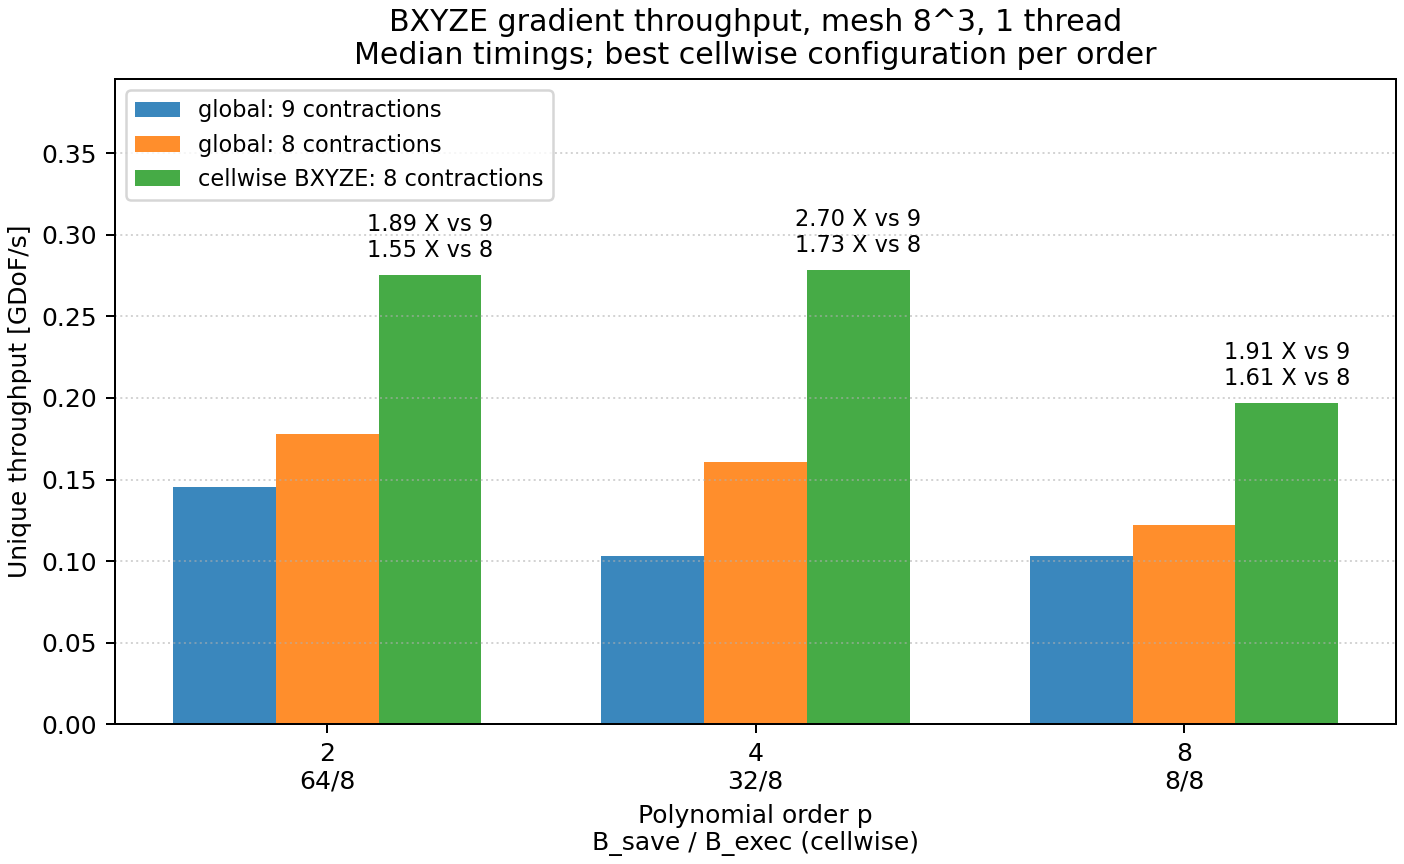
\includegraphics[width=0.96\linewidth]{dss_bxyze_gradient_gdof_s_unique_n8_t1_median.png}
 \par\medskip
 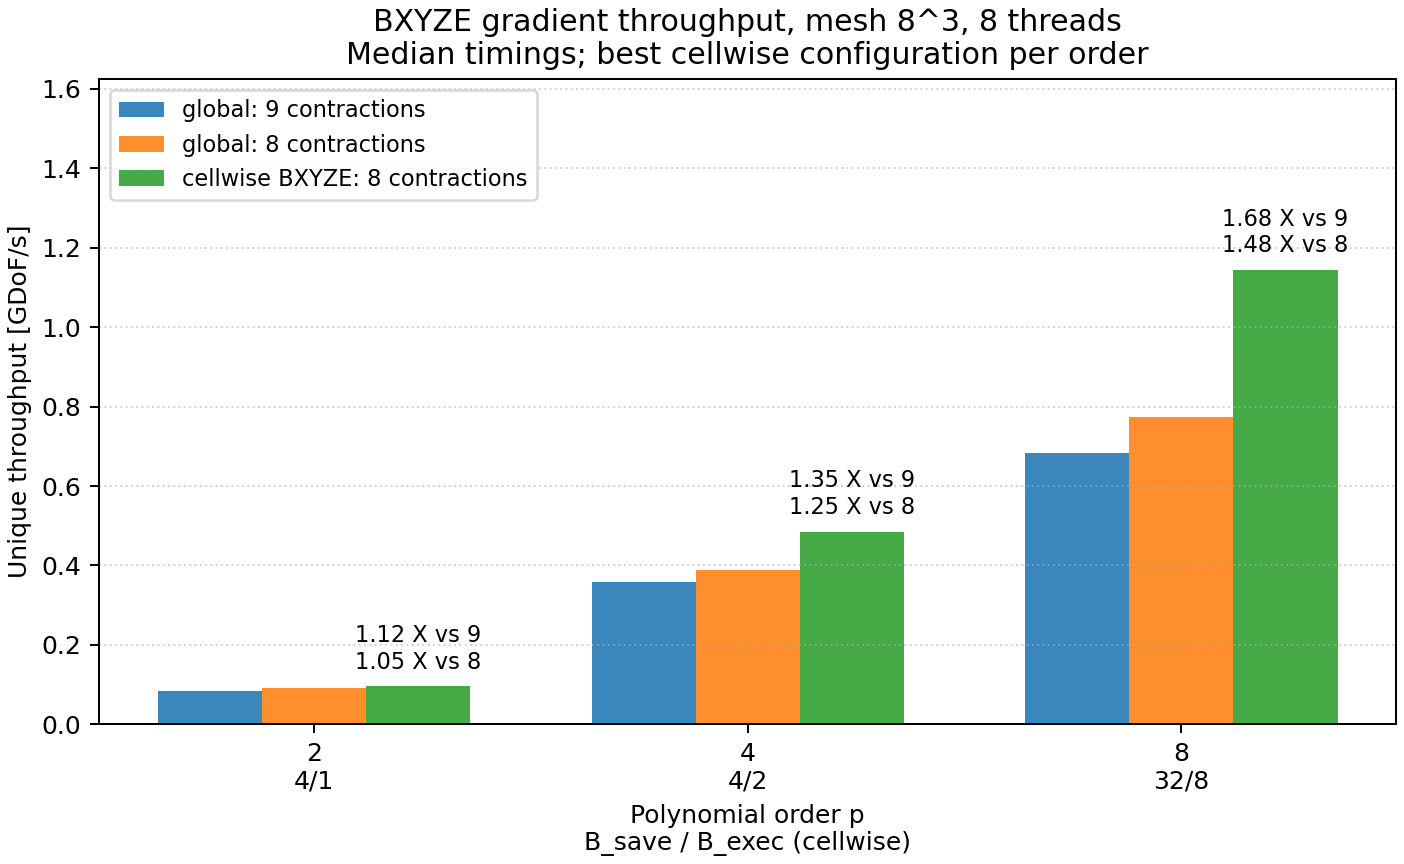
\includegraphics[width=0.96\linewidth]{dss_bxyze_gradient_gdof_s_unique_n8_t8_median.png}
 \caption{Gradient throughput on the \(8^3\)-element macro mesh: one thread
 (top) and eight threads (bottom). Each group compares Global 9, Global 8 and
 cell-wise 8. Tick labels give \(p\) and the selected \(B_s/B_e\); the two
 labels above the cell-wise bar are its speedups against the global references.}
 \label{fig:gradient-throughput-8}
\end{figure}

\begin{figure}[p]
 \centering
 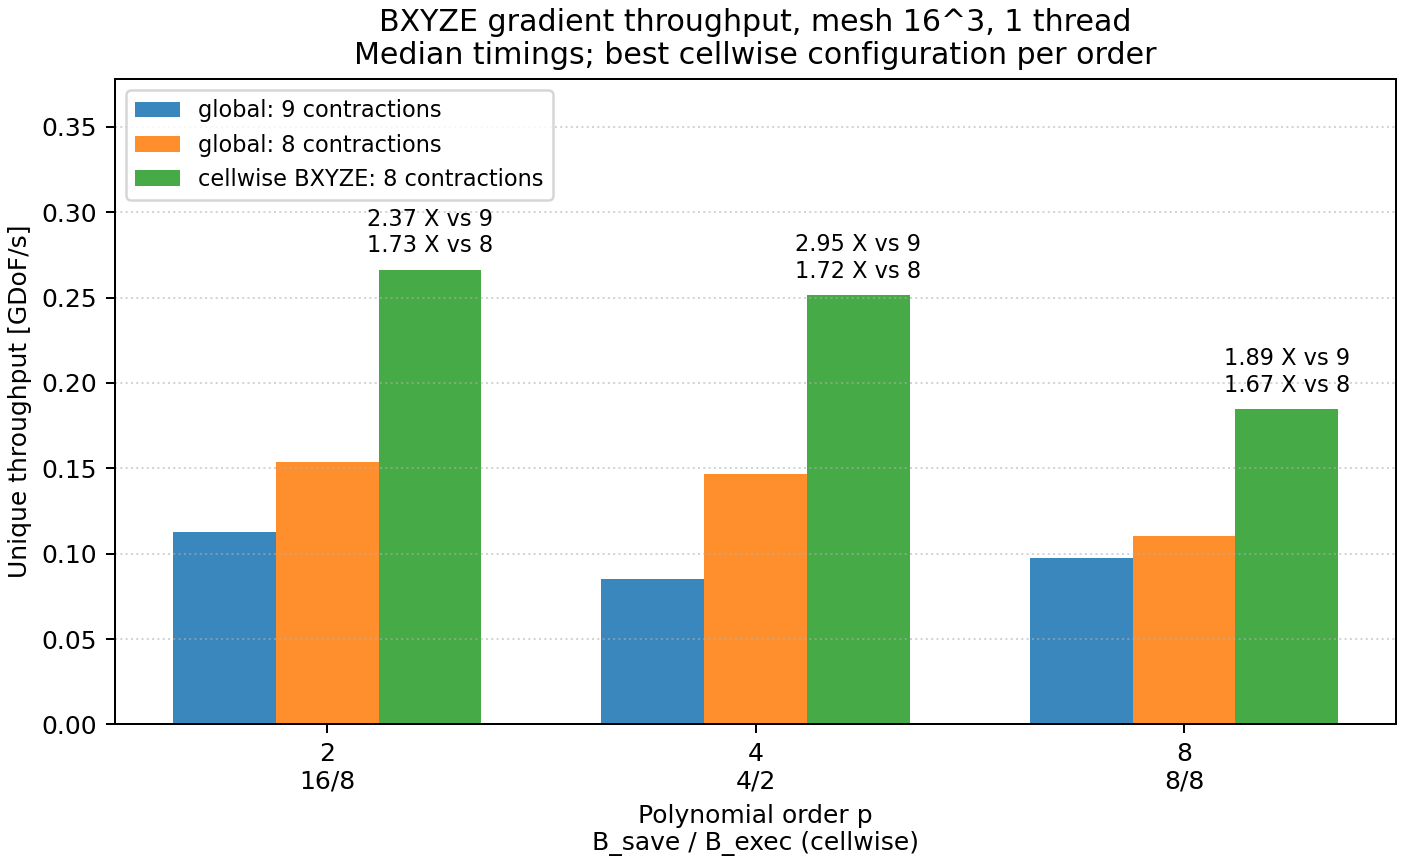
\includegraphics[width=0.96\linewidth]{dss_bxyze_gradient_gdof_s_unique_n16_t1_median.png}
 \par\medskip
 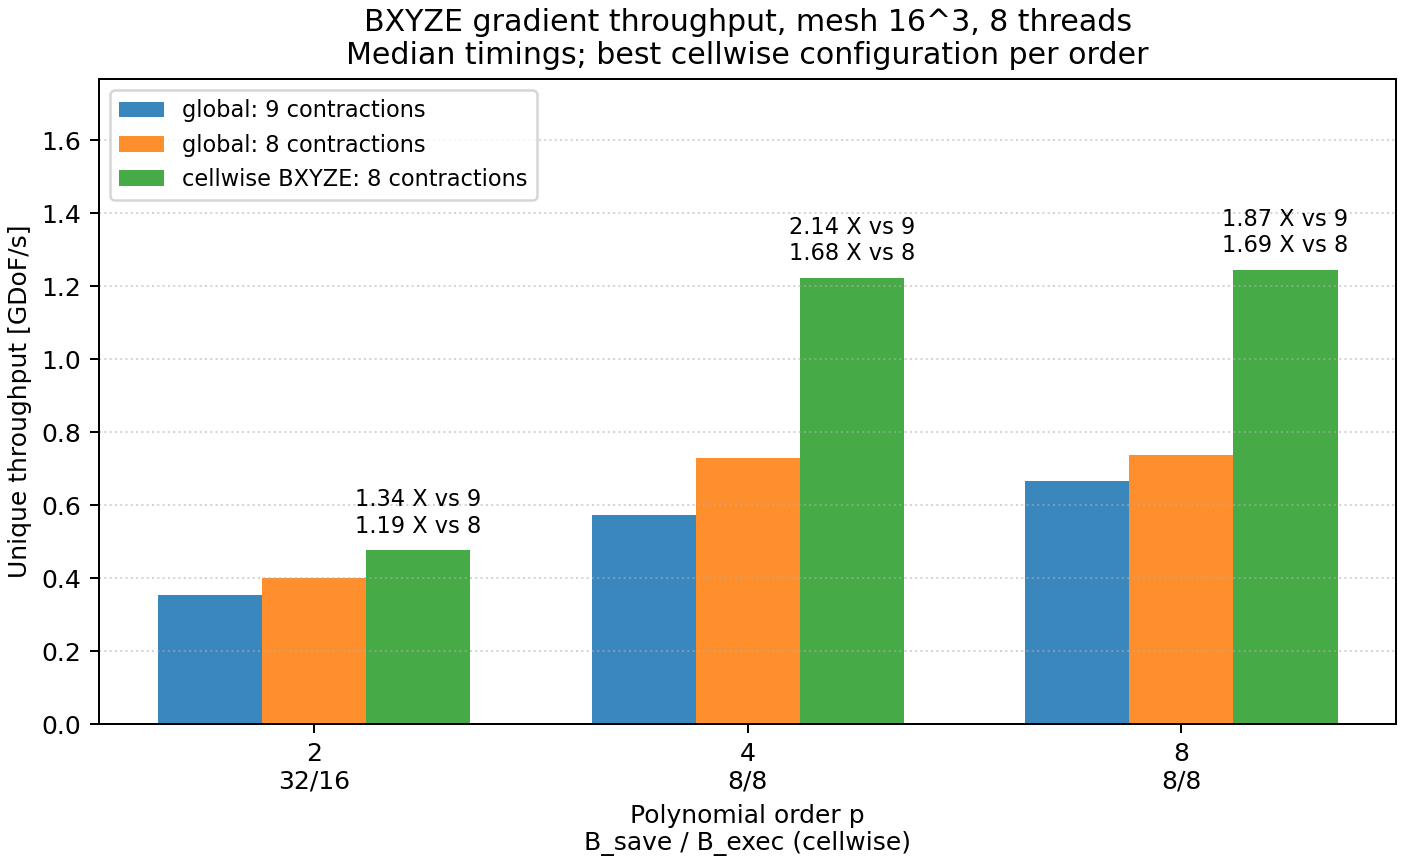
\includegraphics[width=0.96\linewidth]{dss_bxyze_gradient_gdof_s_unique_n16_t8_median.png}
 \caption{The same three-way comparison on the \(16^3\)-element macro mesh,
 with one thread (top) and eight threads (bottom). The retained full-mesh
 gradient writes and the global gathers are included in every measured apply.}
 \label{fig:gradient-throughput-16}
\end{figure}

Table~\ref{tab:gradient-best} records the selected configurations for the larger
mesh. For example, at \(p=8\) with eight threads, the cell-wise path reaches
\(1.244\) GDoF/s, with speedups \(\sigma_9=1.87\) and
\(\sigma_8=1.69\). The second number is the comparison that keeps the
eight-contraction algorithm in both paths.

\begin{table}[htbp]
 \centering\small
 \begin{tabular}{rrrrrrrr}
 \toprule
 Threads & $p$ & $B_s$ & $B_e$ & $\mathcal T_9$ & $\mathcal T_8$
 & $\mathcal T_B$ & $\sigma_8$\\
 \midrule
 1 & 2 & 16 & 8 & 0.113 & 0.154 & 0.266 & 1.73\\
 1 & 4 & 4 & 2 & 0.085 & 0.146 & 0.251 & 1.72\\
 1 & 8 & 8 & 8 & 0.098 & 0.111 & 0.185 & 1.67\\
 \midrule
 8 & 2 & 32 & 16 & 0.356 & 0.402 & 0.477 & 1.19\\
 8 & 4 & 8 & 8 & 0.573 & 0.728 & 1.223 & 1.68\\
 8 & 8 & 8 & 8 & 0.665 & 0.736 & 1.244 & 1.69\\
 \bottomrule
 \end{tabular}
 \caption{Best measured cell-wise configuration per order on the
 \(16^3\)-element macro mesh. All throughputs are in GDoF/s and come from
 median timings of the same configuration row.}
 \label{tab:gradient-best}
\end{table}

\FloatBarrier
\subsection{Sensitivity to storage and execution block sizes}

Figures~\ref{fig:gradient-blocks-8} and~\ref{fig:gradient-blocks-16} show every
measured \((B_s,B_e)\) combination rather than only the best one. Storage block
size varies horizontally, execution batch size vertically, and each panel fixes
the polynomial order. Colors share one throughput scale within each image;
numbers give GDoF/s and the red outline marks the largest value in a panel.
Gray cells are unmeasured combinations, not zero-throughput results.

\begin{figure}[p]
 \centering
 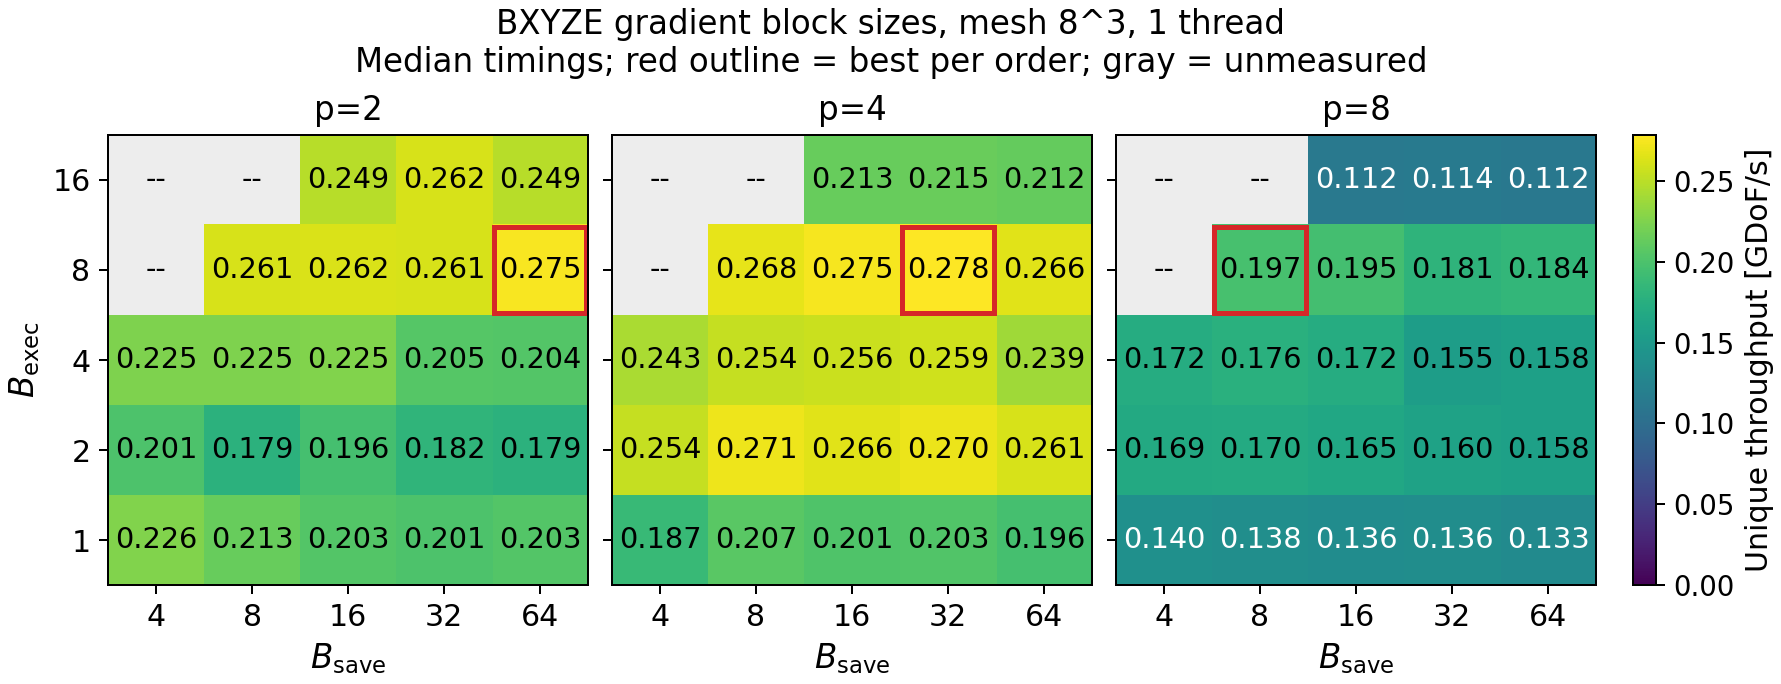
\includegraphics[width=\linewidth]{dss_bxyze_gradient_gdof_s_unique_n8_t1_median_blocks.png}
 \par\bigskip
 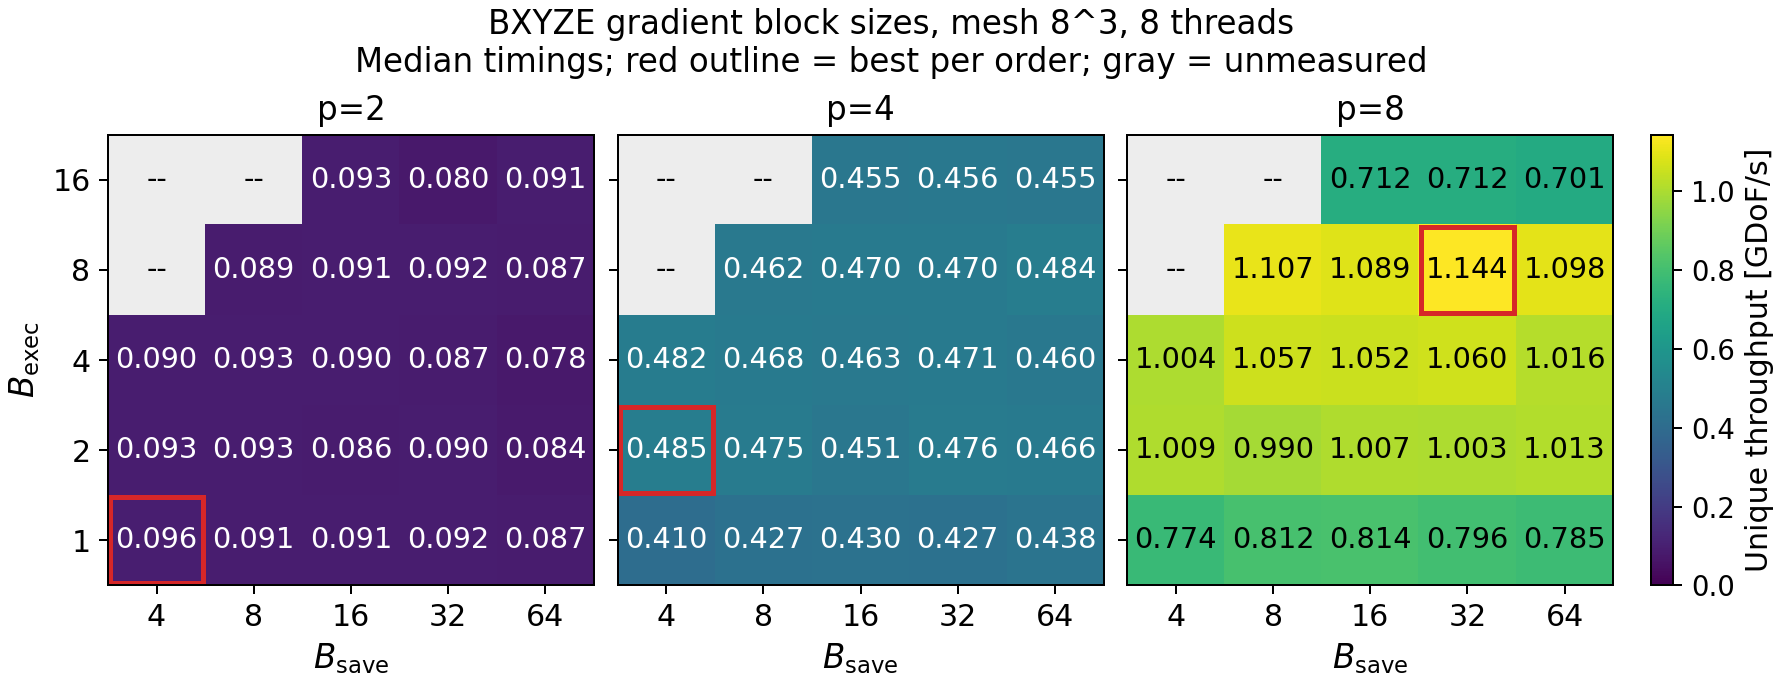
\includegraphics[width=\linewidth]{dss_bxyze_gradient_gdof_s_unique_n8_t8_median_blocks.png}
 \caption{Storage/execution block-size maps for the \(8^3\)-element macro
 mesh, with one thread (top) and eight threads (bottom). Each panel represents
 one order. Gray cells have \(B_e>B_s\) and were not measured.}
 \label{fig:gradient-blocks-8}
\end{figure}

\begin{figure}[p]
 \centering
 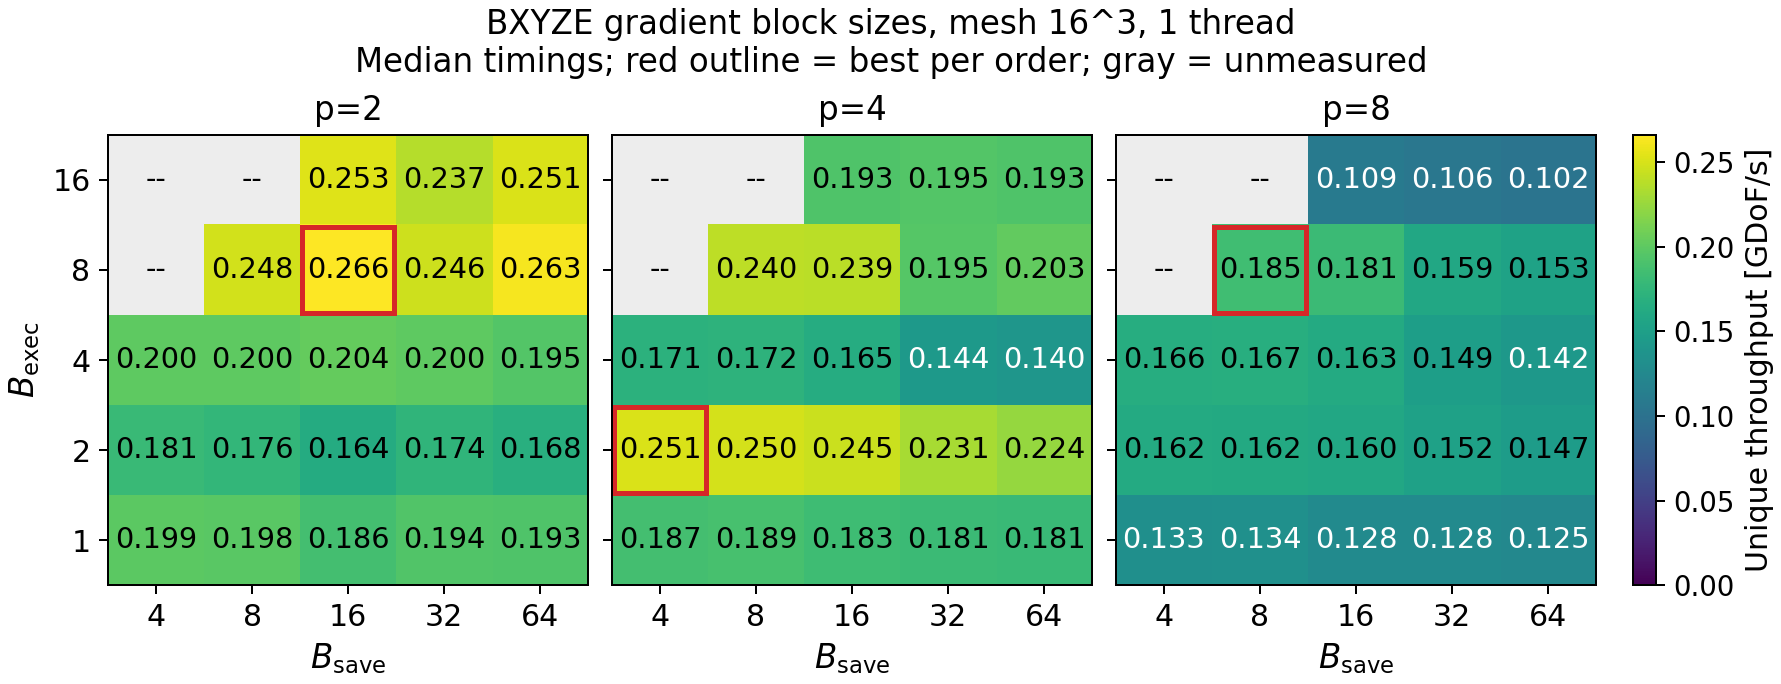
\includegraphics[width=\linewidth]{dss_bxyze_gradient_gdof_s_unique_n16_t1_median_blocks.png}
 \par\bigskip
 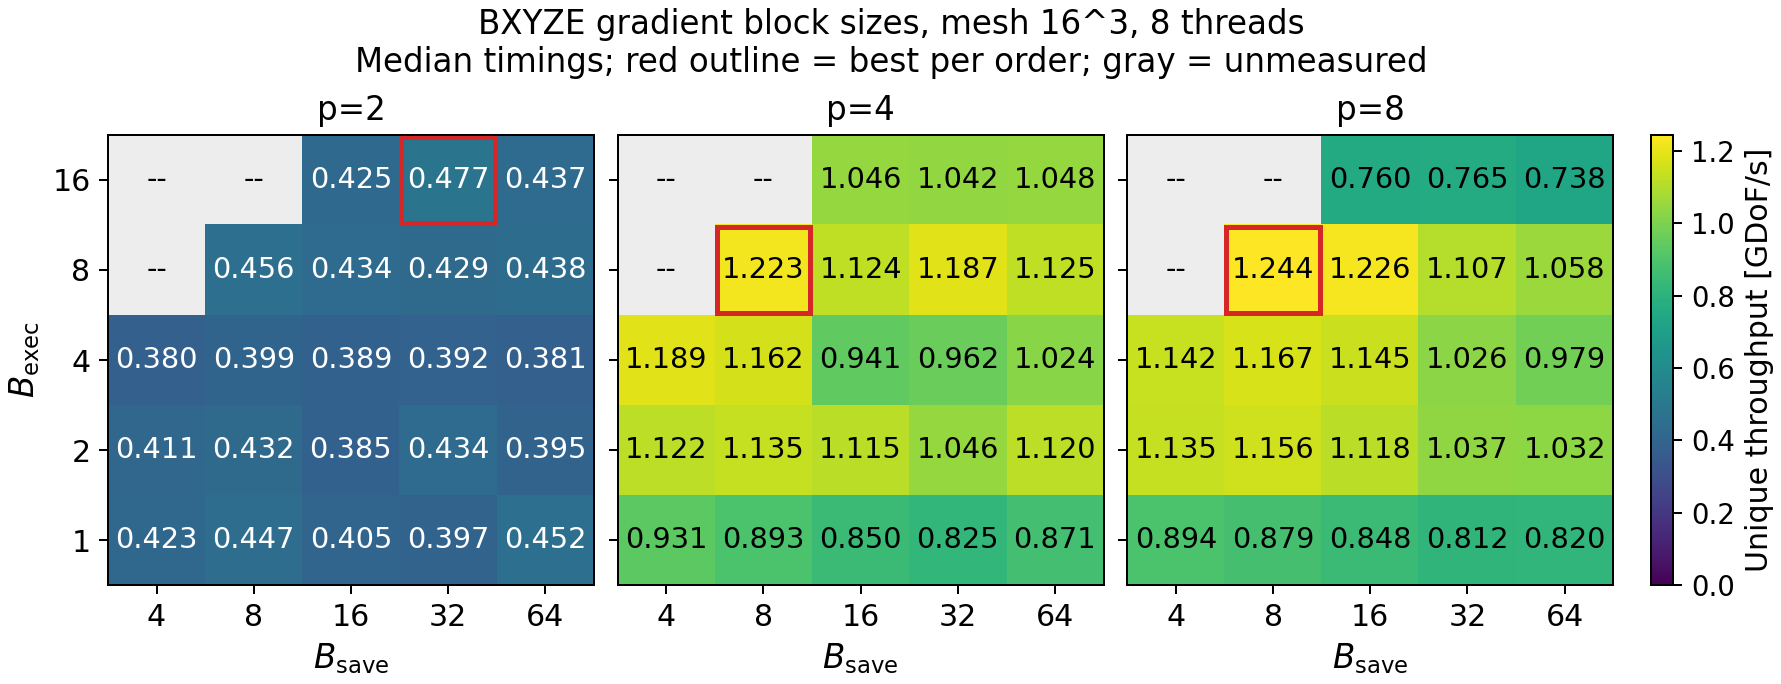
\includegraphics[width=\linewidth]{dss_bxyze_gradient_gdof_s_unique_n16_t8_median_blocks.png}
 \caption{The same parameter maps for the \(16^3\)-element macro mesh.
 The fastest batch size depends on order and thread count; increasing either
 blocking parameter does not guarantee higher throughput.}
 \label{fig:gradient-blocks-16}
\end{figure}

The following comparisons hold one parameter fixed, so they distinguish the
two effects rather than comparing different optima:
\begin{itemize}
 \item \textbf{Changing execution batch size.} On the \(16^3\) mesh at
 \(p=8\), eight threads and fixed \(B_s=16\), throughput for
 \(B_e=1,2,4,8,16\) is approximately
 \(0.848,1.118,1.145,1.226,0.760\) GDoF/s. Larger batches initially help,
 but \(B_e=16\) loses performance. Its explicit scratch is twice that for
 \(B_e=8\), in addition to larger gradient tiles and local accumulator arrays.
 This is consistent with increased cache/register pressure; the timings alone
 do not identify which hardware resource causes the drop.
 \item \textbf{Changing storage block size.} At the same order, mesh and
 thread count with fixed \(B_e=8\), the rates for \(B_s=8,16,32,64\) are
 \(1.244,1.226,1.107,1.058\) GDoF/s. Scratch size is unchanged: increasing
 \(B_s\) changes the input nodal stride, the number of execution batches in
 a storage block and the granularity of the OpenMP block loop.
 \item \textbf{Dependence on order and thread count.} For \(p=4\), the best
 larger-mesh configuration changes from \(B_s/B_e=4/2\) with one thread to
 \(8/8\) with eight threads. A universal choice of the largest batch is not
 supported by this sweep. Lower orders and the smaller mesh also make the
 OpenMP and loop-control costs a larger fraction of an apply.
\end{itemize}

\FloatBarrier
\subsection{Interpretation and subsequent optimizations}

The results compare the three implemented methods under the stated conditions.
The cell-wise input conversion is outside timing, matching the intended
persistent representation. If a workflow converts from a global vector on every
apply, that conversion must be included in its total time. The best block
configuration is selected from the same measurements being plotted; independent
runs with the selected configuration fixed are needed to quantify repeatability.
The six-order schedule balances execution positions, but does not guarantee
identical cache state or core placement. Materializing all gradients also differs
from a fused Laplacian that consumes each batch's gradients immediately.

Eight contractions are an intermediate optimization, not a universal minimum.
For \(Q=N\) with distinct quadrature points, transforming to the nodal basis
at those points and applying its differentiation matrices can use three value
transforms followed by three directional derivatives, giving six transforms in
3D. This does not require the original nodes to coincide with quadrature points.
The approach is described in~\cite{KronbichlerKormann2019} and used in the
transform-to-collocation kernels of deal.II~\cite{dealIIEvaluationKernels}.
That formulation and symmetry/even--odd optimizations remain candidates for
further work. The following section describes the complete Laplacian now
implemented around the eight-contraction gradient and its transpose. The
gradient CSV discussed in this section measures the nine/eight/eight component
comparison only.

\subsection{Files and reproduction}

The relevant implementation files are:
\begin{itemize}
 \item Gradient kernel and workspace query:\\
 {\small\path{operators/dss/sfem_dss_bxyze_affine_laplacian_inline.hpp}}.
 \item Three-method benchmark:\\
 {\small\path{frontend/ops/dss/benchmark/sfem_DSSBXYZEGradientBench.cpp}}.
 \item Measurements:\\
 {\small\path{frontend/ops/dss/benchmark/dss_bxyze_gradient_bench.csv}}.
 \item Polynomial reproduction and scalar-reference checks:\\
 {\small\path{frontend/ops/dss/test/sfem_DSSBXYZEContractionTest.cpp}}.
\end{itemize}

From the repository root, run the compiled benchmark and plot the CSV using a
Python environment containing Matplotlib:
\begin{lstlisting}[language=bash]
PYTHONPATH=python OMPI_MCA_btl=self \
    build/sfem_DSSBXYZEGradientBench

PYTHONPATH=python /path/to/venv/bin/python \
    frontend/ops/dss/benchmark/plot_dss_bxyze_gradient_throughput.py \
    --block-analysis
\end{lstlisting}
The plotting script accepts filters for mesh size, thread count and both block
sizes. Median timings are plotted by default. To plot minimum timings, pass
\texttt{--statistic best}. To generate the parameter maps as well, add
\texttt{--block-analysis}. All figures in this note come from the saved
gradient three-method CSV. The complete-operator measurements below use a
separate driver and CSV.

\FloatBarrier
\section{Affine Cell-wise Laplacian: Setup and Application}
\label{sec:affine-laplacian}

\subsection{Operator and geometric assumptions}

The main entry point is
\texttt{sfem\_dss\_bxyze\_laplacian\_affine\_volumetric\_apply},
implemented in \path{operators/dss/sfem_dss_bxyze_affine_laplacian.cpp}.
It computes the local nodal contributions of the scalar Laplacian in weak form.
Its input and output are persistent BXYZE vectors. It does not construct an
element stiffness matrix.

Let \(\boldsymbol{\xi}\in[0,1]^3\) denote reference coordinates. An affine
element has the mapping
\[
 \boldsymbol{x}=F_e(\boldsymbol{\xi})
 =\boldsymbol{a}_e+J_e\boldsymbol{\xi},
 \qquad \det(J_e)>0,
\]
where \(J_e\) is constant on that element. Such an element is a
parallelepiped: its edges may be rotated, stretched or sheared. Axis alignment
is not required, and different elements may have different Jacobians.
For this mapping,
\[
 \nabla_{\boldsymbol{x}}u=J_e^{-T}\nabla_{\boldsymbol{\xi}}u.
\]
Changing variables in
\(\int_{\Omega_e}\nabla v\cdot\nabla u\,d\boldsymbol{x}\)
therefore gives the symmetric metric
\[
 H_e=\det(J_e)J_e^{-1}J_e^{-T}
 =\begin{pmatrix}
 H_{00}&H_{01}&H_{02}\\
 H_{01}&H_{11}&H_{12}\\
 H_{02}&H_{12}&H_{22}
 \end{pmatrix}.
\]
Only six entries are stored per element. They contain the geometric factor,
including the determinant, but no quadrature weights or material coefficient.
For the unit-coefficient Laplacian, the local operation is
\[
 \boxed{\quad y_e=G^TWH_eGx_e.\quad}
\]
Here \(G\) evaluates the three reference derivatives at the tensor-product
quadrature points, \(H_e\) acts on each three-component gradient, and \(W\)
multiplies by the quadrature weights. The result is a stiffness-operator
contribution, not a pointwise evaluation of the strong Laplacian.
Boundary conditions are handled outside this volume kernel.

This is a partial-assembly approach: the small one-dimensional basis matrices
and six metric entries are prepared once, while tensor contractions are
performed on every apply. Curved or general trilinear hexahedra would require
a metric varying with quadrature position and are outside this implementation.

\subsection{Setup: what is prepared before applying the operator}

The setup has the following stages.
\begin{enumerate}
 \item \textbf{Create the layout.}
 \texttt{sfem\_dss\_bxyze\_create\_layout} records \(p\), \(N=p+1\),
 the element count, \(B_s\) and \(B_e\), and derives the block counts and
 strides. This layout does not require a global structured element ordering.
 The structured dimensions needed by DSS are supplied separately.
 \item \textbf{Prepare quadrature and basis matrices.}
 With \(Q\) points per direction, store
 \[
 S[qN+i]=\ell_i(\xi_q),\qquad
 D[qN+i]=\ell_i'(\xi_q),\qquad
 q_w[q]=w_q.
 \]
 \(S,D\) each contain \(QN\) scalars and are shared by all elements.
 Quadrature coordinates are used to construct them; the apply only needs
 \(S,D\) and the one-dimensional weights.
 \item \textbf{Compute the geometry.}
 \texttt{sfem\_dss\_bxyze\_affine\_geometry} gathers the eight corner
 coordinates, evaluates the metric at the reference center and stores its
 six entries in blocked form. The center value is valid throughout an affine
 element. Affinity is a caller precondition: this routine does not prove that
 a supplied mesh is affine.
 \item \textbf{Prepare execution metadata.}
 \texttt{sfem\_dss\_bxyze\_laplacian\_affine\_volumetric\_setup}
 validates the supported dimensions, copies the layout, calculates the
 per-thread workspace stride and stores a pointer to the selected kernel.
 The switches selecting \(N,Q,B_e,B_s\) run here.
 \item \textbf{Allocate and initialize the persistent data.}
 Allocate the BXYZE input and output, convert the global input using
 \texttt{sfem\_dss\_global\_to\_bxyze}, and allocate one workspace slice per
 OpenMP thread. The output and scratch need no explicit zeroing before apply.
\end{enumerate}
The prepared operator descriptor owns none of these arrays. The caller keeps
them alive, checks setup return codes and supplies disjoint input, output,
geometry and workspace allocations. A schematic allocation and call sequence,
with error handling omitted, is:
\begin{lstlisting}[language=C++]
sfem_dss_bxyze_layout_t layout;
sfem_dss_bxyze_create_layout(p, nelements, B_save, B_exec, &layout);

sfem_dss_bxyze_laplacian_affine_volumetric_t op;
sfem_dss_bxyze_laplacian_affine_volumetric_setup(&layout, Q, &op);

std::vector<scalar_t> geometry(
    sfem_dss_bxyze_affine_geometry_n_values(&layout));
sfem_dss_bxyze_affine_geometry(
    &layout, elements, points, geometry.data());

std::vector<real_t> x(layout.nblocks * layout.block_stride);
std::vector<real_t> y(x.size());
sfem_dss_global_to_bxyze(
    p, nelements, B_save, elements, x_global, x.data());

std::vector<scalar_t> workspace(nthreads * op.workspace_stride);
// S, D and qw have also been prepared before this call.
sfem_dss_bxyze_laplacian_affine_volumetric_apply(
    &op, S.data(), D.data(), qw.data(), geometry.data(),
    x.data(), y.data(), workspace.data());
\end{lstlisting}
Allocate enough slices for the maximum OpenMP team size that will be used by
apply. Changing the team size requires sufficient workspace capacity; changing
the layout or \(Q\) requires a new setup. Changing only input values leaves
basis and geometry data reusable. A mesh-geometry change requires recomputing
the metrics.

For the measured affine, constant-coefficient problem, Gauss--Legendre
quadrature with \(Q=p+1\) is sufficient for exact element integration up to
roundoff. Products of reference basis derivatives have degree at most \(2p\)
in each coordinate, whereas this rule integrates through degree \(2p+1\).
The original equispaced interpolation nodes do not coincide with the
Gauss--Legendre points. Thus \(S\) is not an identity matrix even though
\(Q=N\). The implementation also supports the larger choice \(Q=3p\).

\subsection{Persistent fields, geometry and temporary batch layout}

Use \(v=i_x+N(i_y+Ni_z)\) for the local node index. Within storage block
\(e_b\), let \(\lambda\) be the first lane of an execution batch and
\(0\le b<B_e\) its lane index. The element is \(e=e_bB_s+\lambda+b\).
The three relevant memory offsets are
\[
\begin{aligned}
 I_u&=e_bN^3B_s+vB_s+\lambda+b,\\
 I_H&=(6e_b+c)B_s+\lambda+b,\qquad 0\le c<6,\\
 I_q&=\bigl((q_zQ+q_y)Q+q_x\bigr)B_e+b.
\end{aligned}
\]
The input \(x[I_u]\) and output \(y[I_u]\) have the same persistent layout.
Metric components are ordered
\[
 c=0,\ldots,5:
 \quad H_{00},H_{01},H_{02},H_{11},H_{12},H_{22}.
\]
For example, a storage block holds all \(B_s\) values of \(H_{00}\), then all
\(B_s\) values of \(H_{01}\), and so on. There is no node or quadrature index
in this geometry array. Its total size is \(6B_sn_{\mathrm{blocks}}\) scalars.

Each temporary quadrature component uses the compact layout
\([q_z][q_y][q_x][b]\) with stride \(B_e\). At a fixed tensor point, adjacent
lanes belong to different elements and are contiguous in all three layouts.
The nodal and geometric component strides remain \(B_s\), even when
\(B_e<B_s\). Scratch instead packs only the currently executing batch.

\subsection{Workspace size and lifetime}

The complete operator needs the gradient scratch described in
Section~\ref{sec:sum-factorization}, plus three quadrature buffers.
Set
\[
 C_g=Q^3B_e,\qquad C_x=N^2QB_e,\qquad C_y=NQB_e.
\]
One thread's useful storage is partitioned as follows:
\begin{center}
\begin{tabular}{lll}
\toprule
Region & Starting offset & Scalar values\\
\midrule
\texttt{gx} & \(0\) & \(C_g\)\\
\texttt{gy} & \(C_g\) & \(C_g\)\\
\texttt{gz} & \(2C_g\) & \(C_g\)\\
Shared contraction scratch & \(3C_g\) & \(2C_x+3C_y\)\\
\bottomrule
\end{tabular}
\end{center}
Consequently,
\[
 W_{\mathrm{useful}}
 =B_e(3Q^3+2N^2Q+3NQ).
\]
The public workspace query and setup include the thread-separation gap:
\[
 g=\frac{128}{\operatorname{sizeof}(\texttt{scalar\_t})},
 \qquad
 \texttt{workspace\_stride}
 =\left(\left\lceil\frac{W_{\mathrm{useful}}}{g}\right\rceil+1\right)g.
\]
These counts are scalar values, not bytes. For \(T\) threads, allocate
\(T\,\texttt{workspace\_stride}\) values; thread \(t\) starts at
\(\texttt{workspace}+t\,\texttt{workspace\_stride}\).
The gap separates active slices but does not specify allocation-base alignment.

The buffers have three consecutive lifetimes. Forward evaluation fills
\texttt{gx,gy,gz}; metric application replaces those values with weighted
fluxes; transpose evaluation reads the fluxes and reuses the forward scratch.
The next batch overwrites everything it needs. In particular, the transpose
seeds its accumulations on the first \(q_y\) slice, so it does not read
uninitialized scratch or require a separate clearing pass.
There are also small local lane accumulators inside the helpers.

The workspace scales with threads and \(B_e\), not with mesh size or \(B_s\).
For \(p=8\), \(Q=N=9\), the useful storage is \(121.5\), \(243\) and
\(486\) KiB per thread at \(B_e=4,8,16\), respectively, in double precision.
The allocated stride adds \(0.125\) KiB in these cases. Thus wider batches
also increase the working set; they do not automatically improve throughput.

\subsection{Main loop and first sum factorization}

The public apply checks its required pointers and calls the prepared function
pointer. It does not recalculate workspace size or repeat dimension dispatch.
The selected implementation is \texttt{volumetric\_apply\_tpl}. It enters one
OpenMP parallel region, obtains each thread's workspace slice and distributes
storage blocks using \texttt{schedule(static)}. Inside that region, the
essential loop is:
\begin{lstlisting}[language=C++]
for (ptrdiff_t eb = 0; eb < layout.nblocks; ++eb) {
    for (int lane = 0; lane < B_save; lane += B_EXEC) {
        const real_t *xb = x + eb * block_stride + lane;
        const scalar_t *h = geometry + eb * (6 * B_save) + lane;
        real_t *yb = y + eb * block_stride + lane;

        sfem_dss_bxyze_lagrange_gradient<N, Q, B_EXEC>(
            B_save, S, D, xb, gx, gy, gz, scratch);
        sfem_dss_bxyze_affine_metric_apply<Q, B_EXEC>(
            B_save, qw, h, gx, gy, gz);
        sfem_dss_bxyze_lagrange_gradient_transpose<N, Q, B_EXEC>(
            B_save, S, D, gx, gy, gz, yb, scratch);
    }
}
\end{lstlisting}
The outer loop identifies the storage block; the inner loop visits its
\(B_s/B_e\) execution batches. For \(B_s=16,B_e=4\), its starting lanes are
\(0,4,8,12\). A thread processes these four batches sequentially, while other
threads own different blocks. No threads cooperate on a single batch.

The first helper is the eight-contraction gradient already described:
\[
\begin{aligned}
 s_x&=S_xx_e,& d_x&=D_xx_e,\\
 a_x&=S_yd_x,& a_y&=D_ys_x,& a_z&=S_ys_x,\\
 g_x&=S_za_x,& g_y&=S_za_y,& g_z&=D_za_z.
\end{aligned}
\]
These are derivatives in reference coordinates, not physical-coordinate
gradients. The x stage fills two \(N^2QB_e\) buffers. The y and z stages
stream one \(q_y\) slice at a time through three \(NQB_e\) buffers, producing
the complete \(Q^3B_e\) arrays for each derivative.
Only this batch's gradients are retained. The main loop immediately consumes
them before moving to the next batch, instead of materializing quadrature
gradients for the entire mesh as the component benchmark does.

\subsection{Metric application and quadrature weights}

For every quadrature point, form
\[
 w_q=q_w[q_x]q_w[q_y]q_w[q_z],\qquad
 \boldsymbol{f}_q=w_qH_e\boldsymbol{g}_q.
\]
The three component updates are
\[
\begin{aligned}
 f_x&=w_q(H_{00}g_x+H_{01}g_y+H_{02}g_z),\\
 f_y&=w_q(H_{01}g_x+H_{11}g_y+H_{12}g_z),\\
 f_z&=w_q(H_{02}g_x+H_{12}g_y+H_{22}g_z).
\end{aligned}
\]
The metric helper loops over \(q_z,q_y,q_x\), then over the batch lanes.
Each weight product is shared across the lanes. For each metric component,
the lane loop reads contiguous values across the batch; the six components
of one element remain separated by stride \(B_s\). A lane saves its three
gradient values in local variables and overwrites the corresponding
\texttt{gx,gy,gz} entries with \(f_x,f_y,f_z\).
Saving all three old components before any store is
necessary because each flux depends on all three gradients.
No additional flux allocation is needed, and weights are applied exactly once.

Although the six metrics are constant over the element, the current code
references them inside the quadrature loop. Their small batch working set is
reused across quadrature points; these references do not imply a fresh DRAM
transfer every time. Compiler hoisting and register retention depend on the
generated code. The implementation does not explicitly reserve registers for
all six components across the complete quadrature traversal.

\textbf{A next step is to fuse this operation into the first sum
factorization.} At the end of its z contraction, a lane already has all three
reference-gradient components for one quadrature point in local accumulators.
Instead of storing those gradients, the helper could immediately multiply by
\(w_qH_e\) and store the three weighted fluxes. The transpose would then read
those flux buffers directly.
This would remove the separate metric sweep and its intermediate gradient
stores and reloads. The three flux buffers would still be needed by the
current transpose schedule, and this traffic saving concerns the memory
hierarchy, not necessarily DRAM alone. Introducing the metric computation at
that point may also increase live values and register pressure. It is a
proposed optimization to benchmark, not a change already included in the
results below.

\subsection{Transpose sum factorization and nodal output}

The final helper applies the algebraic transpose of the gradient graph to
the weighted fluxes. With \(A,B,C\) denoting temporary arrays, its schedule is
\[
\begin{aligned}
 A&=S_z^Tf_x,&B&=S_z^Tf_y,&C&=D_z^Tf_z,\\
 \widetilde d_x&=S_y^TA,&
 \widetilde s_x&=D_y^TB+S_y^TC,\\
 y_e&=D_x^T\widetilde d_x+S_x^T\widetilde s_x.
\end{aligned}
\]
This is \(3+3+2=8\) directional contractions. The two contributions to
\(\widetilde s_x\) are combined before the final x interpolation, reversing
the forward reuse of \(S_xx_e\). Applying three independent transpose tensor
products would instead require nine contractions.

The implementation streams one \(q_y\) plane: three z contractions fill
three \([i_z][q_x][b]\) arrays, then the y stage accumulates into two
\([i_z][i_y][q_x][b]\) arrays. After all \(q_y\) slices, the two x contractions
are summed and written once per node into the persistent BXYZE output.
The temporary shapes are the same as those of the forward scratch, so both
helpers share one allocation.

The basis arrays retain their forward storage \(S[qN+i]\), \(D[qN+i]\).
The transpose changes which index is summed: it reduces over \(q\) and
produces nodal index \(i\). No transposed matrices are constructed and no
quadrature weights are applied again.
The output uses nodal stride \(B_s\), even though the temporary buffers use
\(B_e\). Every element-local output is overwritten, so repeated applies compute
a new result rather than accumulate the previous one. Input and output must
be disjoint; in-place application is not supported.

\subsection{Local contributions and the DSS step}

Let \(R\) copy a unique global vector into the cell-wise representation, and
let \(A_{\mathrm{cell}}\) contain the independent element operators. The
relationship to global assembly is
\[
 x_{\mathrm{cell}}=Rx_{\mathrm{global}},\qquad
 y_{\mathrm{local}}=A_{\mathrm{cell}}x_{\mathrm{cell}},\qquad
 y_{\mathrm{global}}=R^Ty_{\mathrm{local}}.
\]
The volume apply stops at \(y_{\mathrm{local}}\). Copies of a shared node
contain different element contributions at that point.
The DSS operation produces
\[
 y_{\mathrm{DSS}}=RR^Ty_{\mathrm{local}},
\]
so every copy of a shared node receives the same assembled sum.
It is summation, not averaging. Once DSS has been applied, scatter-adding
all copies again would count shared values multiple times.

The current call is
\texttt{sfem\_dss\_bxyze\_structured\_inplace}, implemented in
\path{operators/dss/sfem_dss_bxyze_structured.cpp}.
It requires a logical \(n_x\times n_y\times n_z\) grid, consistently oriented
local tensor axes and element ordering
\[
 e=e_x+n_x(e_y+n_ye_z).
\]
Its successive z, y and x face-summation phases also propagate the sums
through shared edges and corners. It uses this topology rather than physical
coordinates, so a compatible mesh may be graded and sheared; it need not be
axis aligned. Arbitrary unstructured adjacency or rotated local face
orientations need a more general DSS implementation.

This separates two requirements: the volume kernel works with affine metrics
in any element order consistent across its arrays, while the present DSS
requires the specified structured connectivity and ordering.
In the benchmark, apply and DSS are separate calls with separate OpenMP
parallel regions; that overhead is included in apply+DSS timing.

\subsection{Batching, SIMD and current implementation scope}

At each tensor point the innermost loop runs over \(B_e\) independent elements,
with \texttt{omp simd} annotations. There is no reduction between elements.
Basis coefficients and weight products are shared across lanes, while field
values and metric components vary by lane. This is the main SIMD opportunity
provided by BXYZE.

Setup selects fixed \(N,Q,B_e\), and fixed storage strides for
\(B_s\in\{1,2,4,8,16,32,64\}\). The three numerical helpers are forced inline
so those constants can propagate into their loops. Other valid \(B_s\) values
use a generic storage-stride path. There is still a prepared function-pointer
call at the public entry point, but no dimension switches inside each batch.
The volume apply does not read connectivity or physical coordinates, perform
a global gather/scatter, allocate heap storage or synchronize shared nodal
values. Those responsibilities belong to setup and DSS.

The supported degrees are \(p\in\{2,4,8\}\), with \(Q=N\) or \(Q=3p\), and
\(B_e\in\{1,2,4,8,16\}\). The current complete operator requires
\[
 B_e\le B_s,\qquad B_s\bmod B_e=0,\qquad
 n_{\mathrm{elements}}\bmod B_s=0.
\]
Thus all its batches and storage blocks are full. Conversion and geometry
creation can fill padded lanes with zero, but complete-operator setup currently
rejects a partial final storage block. Support for that tail is future work.
The separate gap between thread slices is already included in the workspace.

Fixed bounds and contiguous lanes make vectorization possible; they do not
guarantee that every generated loop uses SIMD or that the widest batch is
fastest. Larger \(B_e\) increases explicit scratch and local accumulators.
Changing \(B_s\) changes nodal strides, batches per block and OpenMP scheduling
granularity, while leaving useful per-batch workspace unchanged.
These parameters therefore need measurement on the target machine.

\subsection{Complete-operator benchmark and measurement boundaries}

The driver is
\path{frontend/ops/dss/benchmark/sfem_DSSBXYZEAffineLaplacianGlobalBench.cpp}.
It constructs graded, sheared meshes with structured logical connectivity.
Starting from macro-grid coordinates \(x,y,z\), it sets
\[
\begin{aligned}
 a&=x+0.125x^2,&b&=0.75y+0.0625y^2,&c&=0.5z+0.03125z^2,\\
 \boldsymbol{x}_{\mathrm{physical}}
 &=\bigl(a+0.25b-0.125c,\ b+0.125c,\ c\bigr).
\end{aligned}
\]
The separable grading defines unequal axis intervals; the subsequent fixed
shear maps each logical cell to an affine parallelepiped.
Consequently the benchmark exercises element-dependent metrics and
off-diagonal components while remaining compatible with the structured DSS.
The semi-structured conversion preserves the required element ordering.

All paths use the same random global input, with seed 42, and the same
Gauss--Legendre rule \(Q=p+1\). The driver compares:
\begin{enumerate}
 \item \textbf{Global 8.} Zero the unique global output; for each element,
 gather its nodal input into a preallocated contiguous buffer, apply the
 eight-contraction gradient, affine metric and eight-contraction transpose,
 then scatter-add the local result. Geometry is precomputed here too.
 The scatter is serial with one thread and atomic with multiple threads.
 This baseline calls the same numerical helpers with \(B_e=1\) and storage
 stride 1; it is not the earlier nine-contraction gradient path.
 \item \textbf{Cell-wise apply.} Call the public batched volume apply,
 reading and overwriting persistent BXYZE arrays. Its output contains local
 contributions before assembly.
 \item \textbf{Cell-wise apply+DSS.} Call the same volume apply and
 immediately perform structured DSS on its output. Every cell copy then
 matches the assembled global result at the corresponding global node.
\end{enumerate}
The apply-only comparison isolates the local operator and layout effects.
The apply+DSS comparison is the one that includes assembly on both sides.
The global baseline's atomic scatter is one implementation choice; these
measurements do not establish performance against other global assembly
strategies such as coloring.

Setup, basis evaluation, geometry computation, input conversion, allocation,
correctness checks and CSV writes are outside timing. All timed paths include
their field reads, intermediate reads/writes, output stores and OpenMP
synchronization. Global output zeroing is timed because its scatter
accumulates; BXYZE output zeroing is unnecessary because the volume kernel
overwrites it. The apply+DSS time includes the two public calls and their
parallel-region costs.

The saved sweep uses Apple M4 Pro code generation, double-precision fields
and arithmetic, \(p\in\{2,4,8\}\), macro meshes of \(16^3\) and \(64^3\)
elements, and one or eight OpenMP threads. It tests
\[
 B_s\in\{1,2,4,8,16,32,64\},\qquad
 B_e\in\{1,2,4,8,16\},
\]
retaining the 25 valid pairs. This gives
\(3\times2\times2\times25=300\) configurations.
The \(16^3\) problems use six warm-up rounds and 12 timed rounds; the
\(64^3\) problems use one warm-up round and six timed rounds.
Timed rounds cycle through all six permutations of the three methods, so
each method occupies each timing position equally often.
Dynamic OpenMP team sizing is disabled and actual thread counts are checked;
core placement is left to the operating system and runtime.

Before timing, each batched local result is compared with a \(B_s=B_e=1\)
reference, and every post-DSS cell copy is compared with global assembly.
Assembly is checked again after repeated calls. The final 300-row dataset
has maximum observed local absolute difference zero and assembled absolute
difference \(8.8818\times10^{-16}\). Atomic accumulation order may vary, so
bitwise equality with global assembly is not a requirement.

\subsection{Throughput, block selection and results}

As for the gradient benchmark, throughput counts unique global DoFs:
\[
 \mathcal T=10^{-9}\frac{n_{\mathrm{global\,DoFs}}}{t},
 \qquad n_{\mathrm{global\,DoFs}}=(pn+1)^3
\]
for an \(n^3\) macro mesh. The duplicated cell-wise count \(n^3(p+1)^3\)
is not used in this numerator.
The CSV stores minimum and median wall times, corresponding throughputs,
paired speedups, errors and independent flags for the fastest apply and
apply+DSS configurations.

Figures~\ref{fig:affine-throughput-16} and
\ref{fig:affine-throughput-64} use medians and select the two cell-wise
configurations independently for each problem. To obtain a single global
bar independent of either winner, the plotting script takes the median of
the 25 recorded global median times. Calling that time \(t_G\), and the
selected cell-wise median times \(t_A,t_D\), the displayed labels are
\[
 \sigma_A=t_G/t_A,\qquad \sigma_D=t_G/t_D.
\]
They are recomputed against that common baseline and may differ from the
paired speedups stored in a winning CSV row. This aggregation differs from
the earlier gradient figures, which use their winning row's references.
The tick labels give \(B_s/B_e\) for apply, followed by \(B_s/B_e\) for
apply+DSS.

\begin{figure}[p]
 \centering
 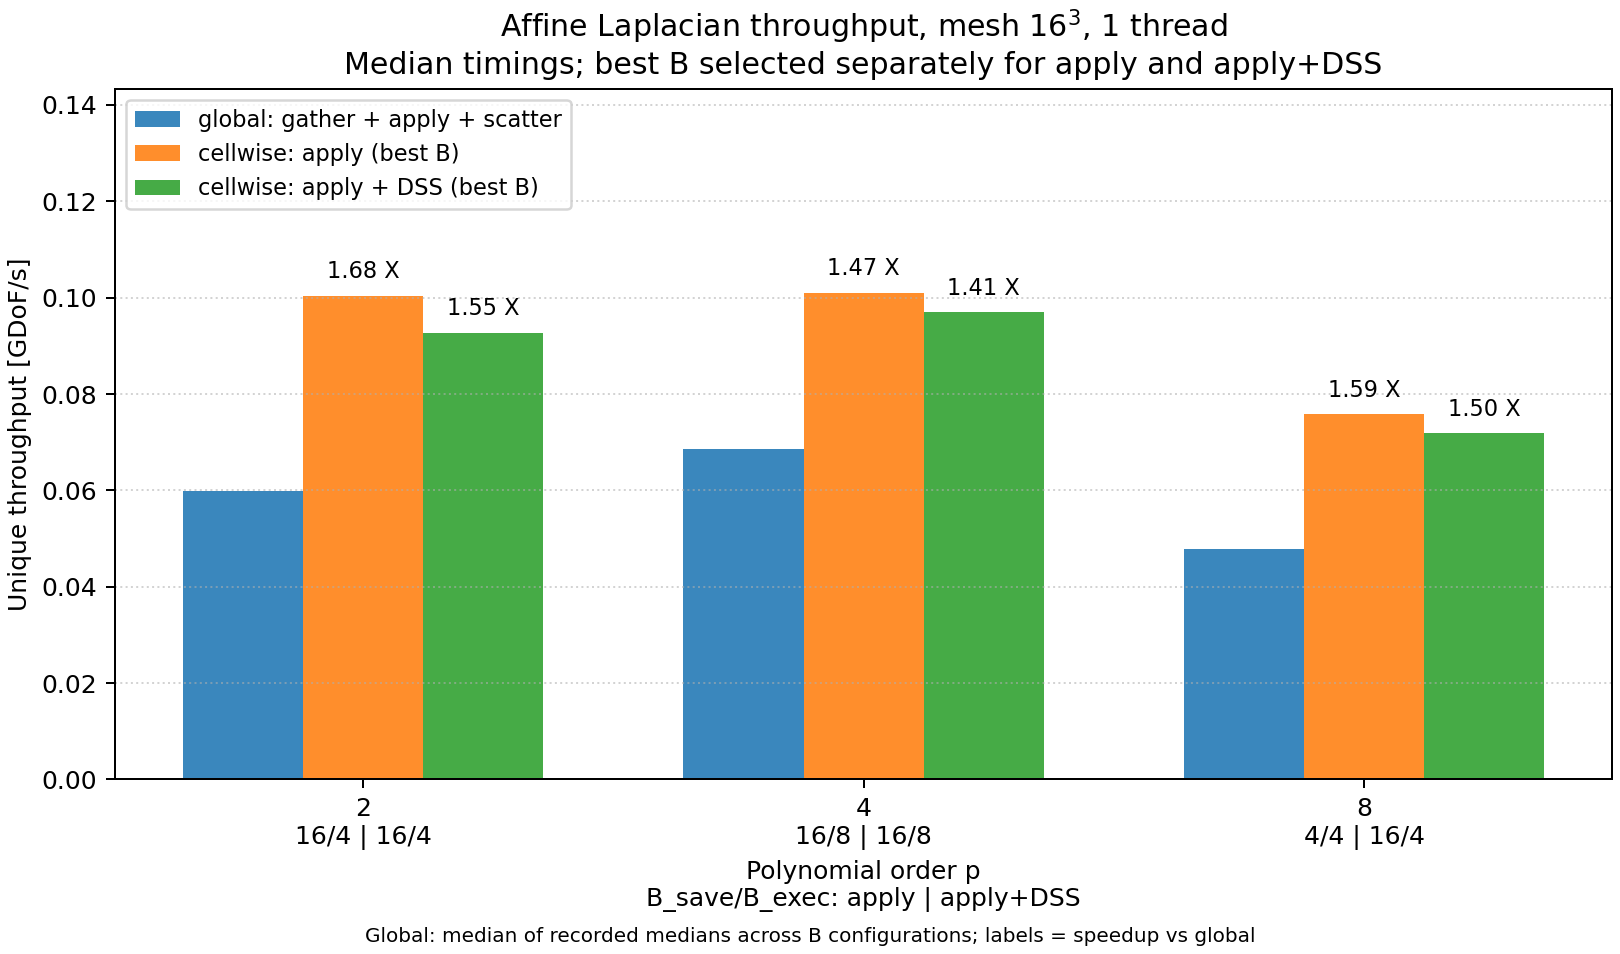
\includegraphics[width=0.96\linewidth]{dss_bxyze_affine_laplacian_global_gdof_s_unique_n16_t1_median.png}
 \par\medskip
 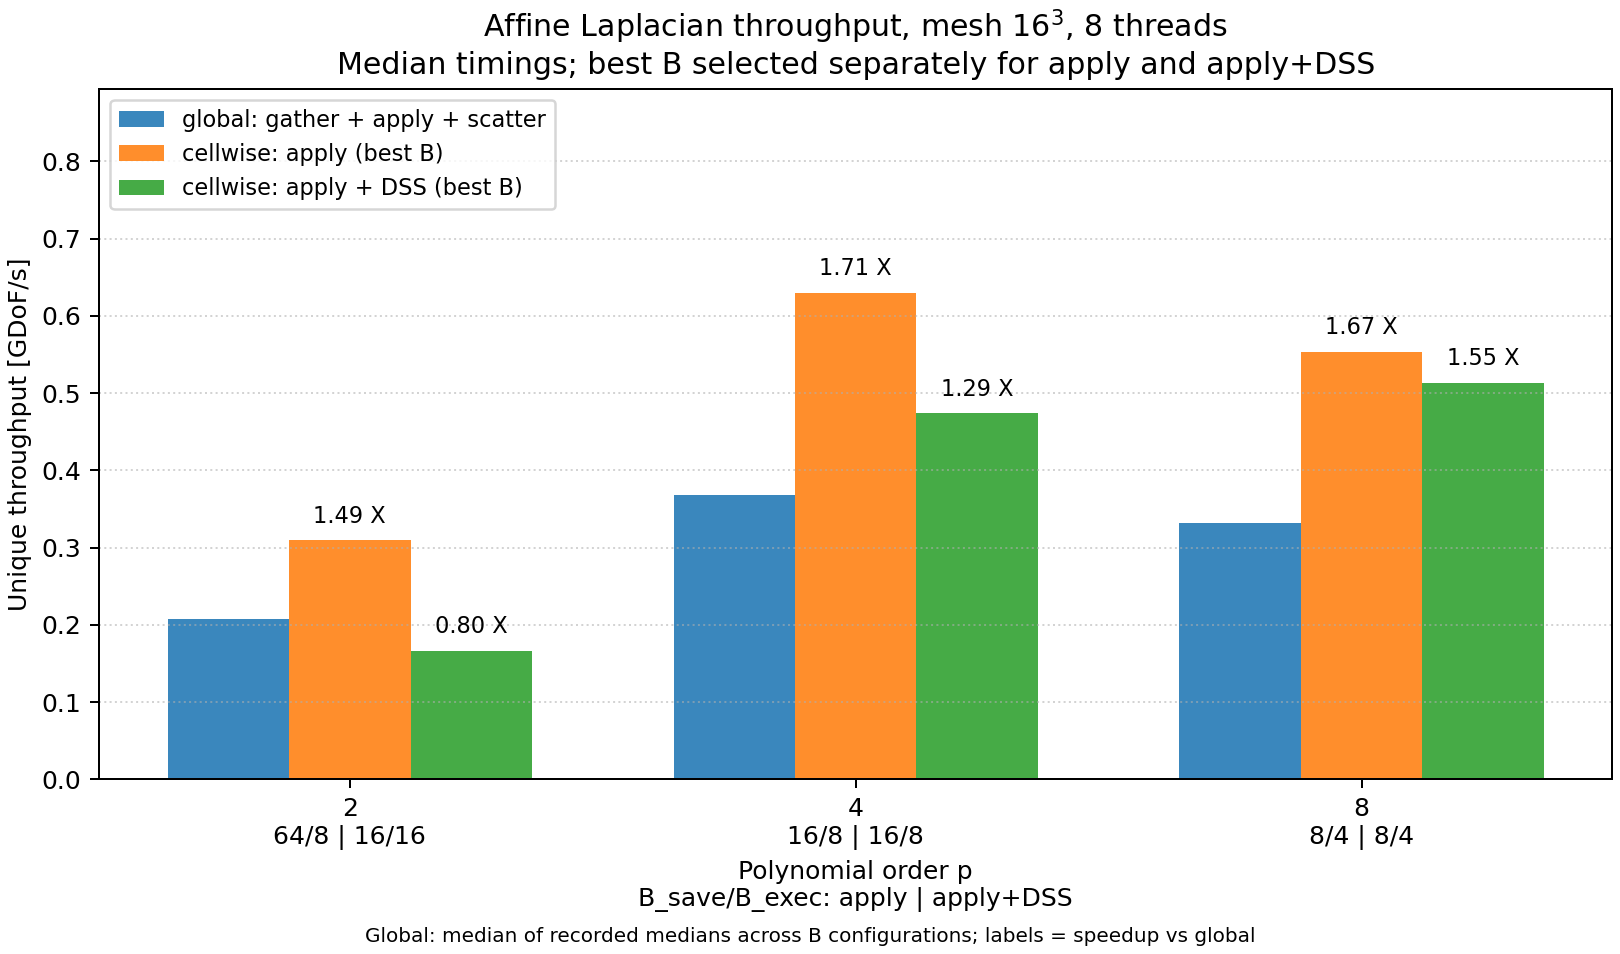
\includegraphics[width=0.96\linewidth]{dss_bxyze_affine_laplacian_global_gdof_s_unique_n16_t8_median.png}
 \caption{Complete affine Laplacian throughput on the \(16^3\)-element macro
 mesh, with one thread (top) and eight threads (bottom). Blue includes global
 zeroing, gather, local apply and scatter; orange stops at local BXYZE output;
 green includes DSS. The two cell-wise block choices are selected separately.}
 \label{fig:affine-throughput-16}
\end{figure}

\begin{figure}[p]
 \centering
 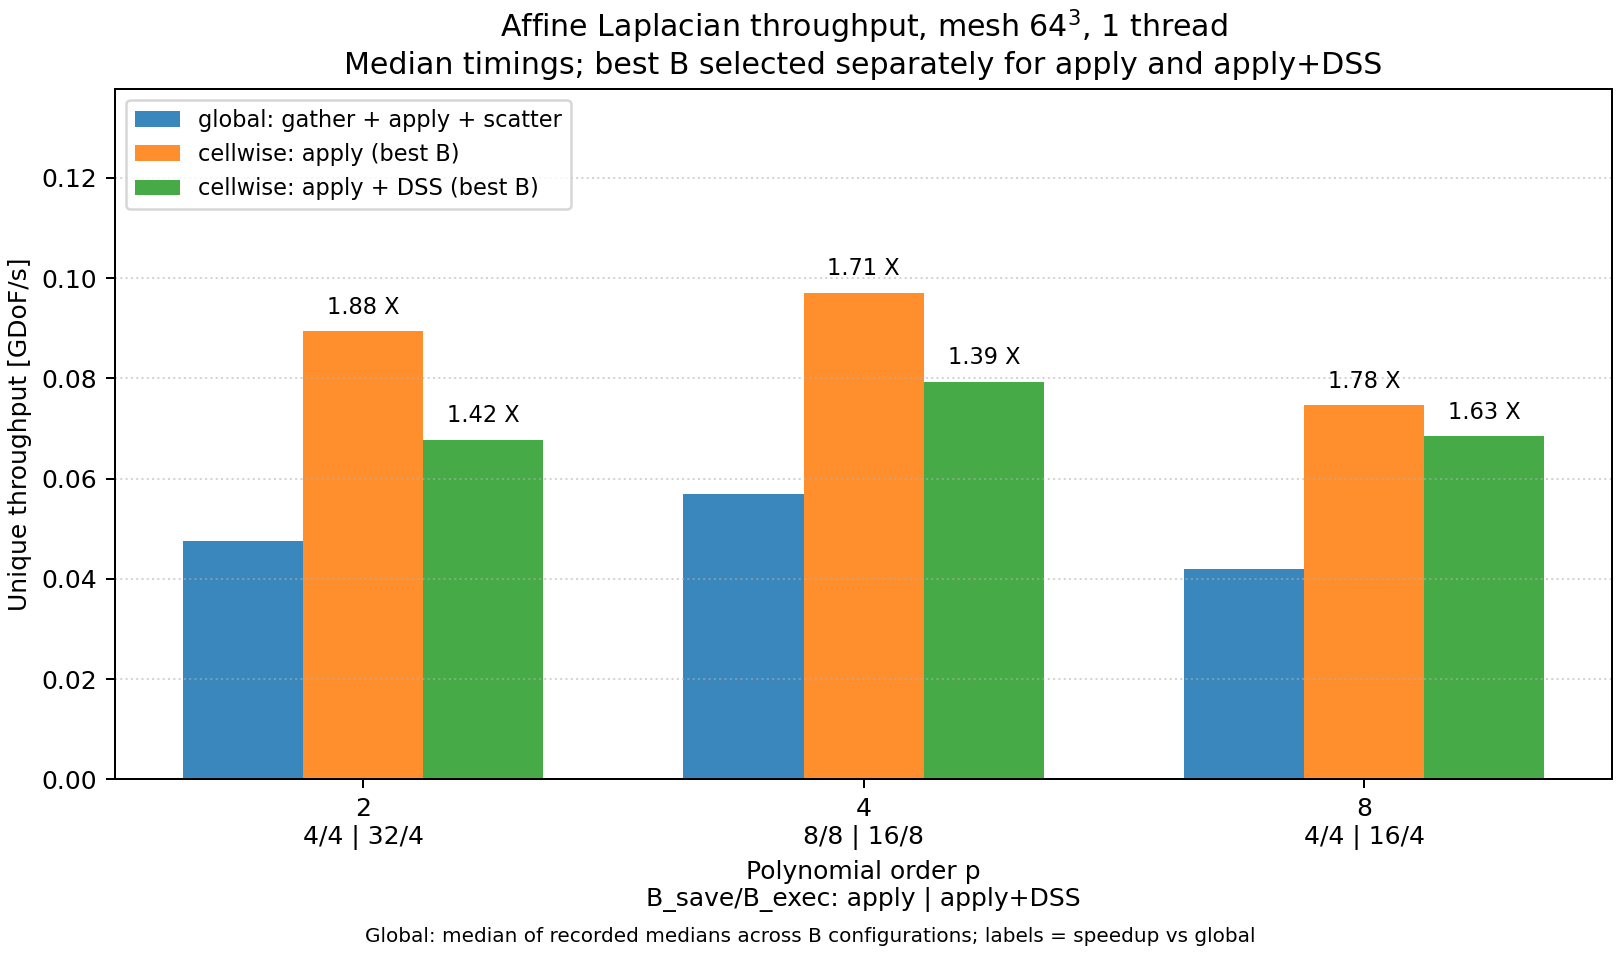
\includegraphics[width=0.96\linewidth]{dss_bxyze_affine_laplacian_global_gdof_s_unique_n64_t1_median.png}
 \par\medskip
 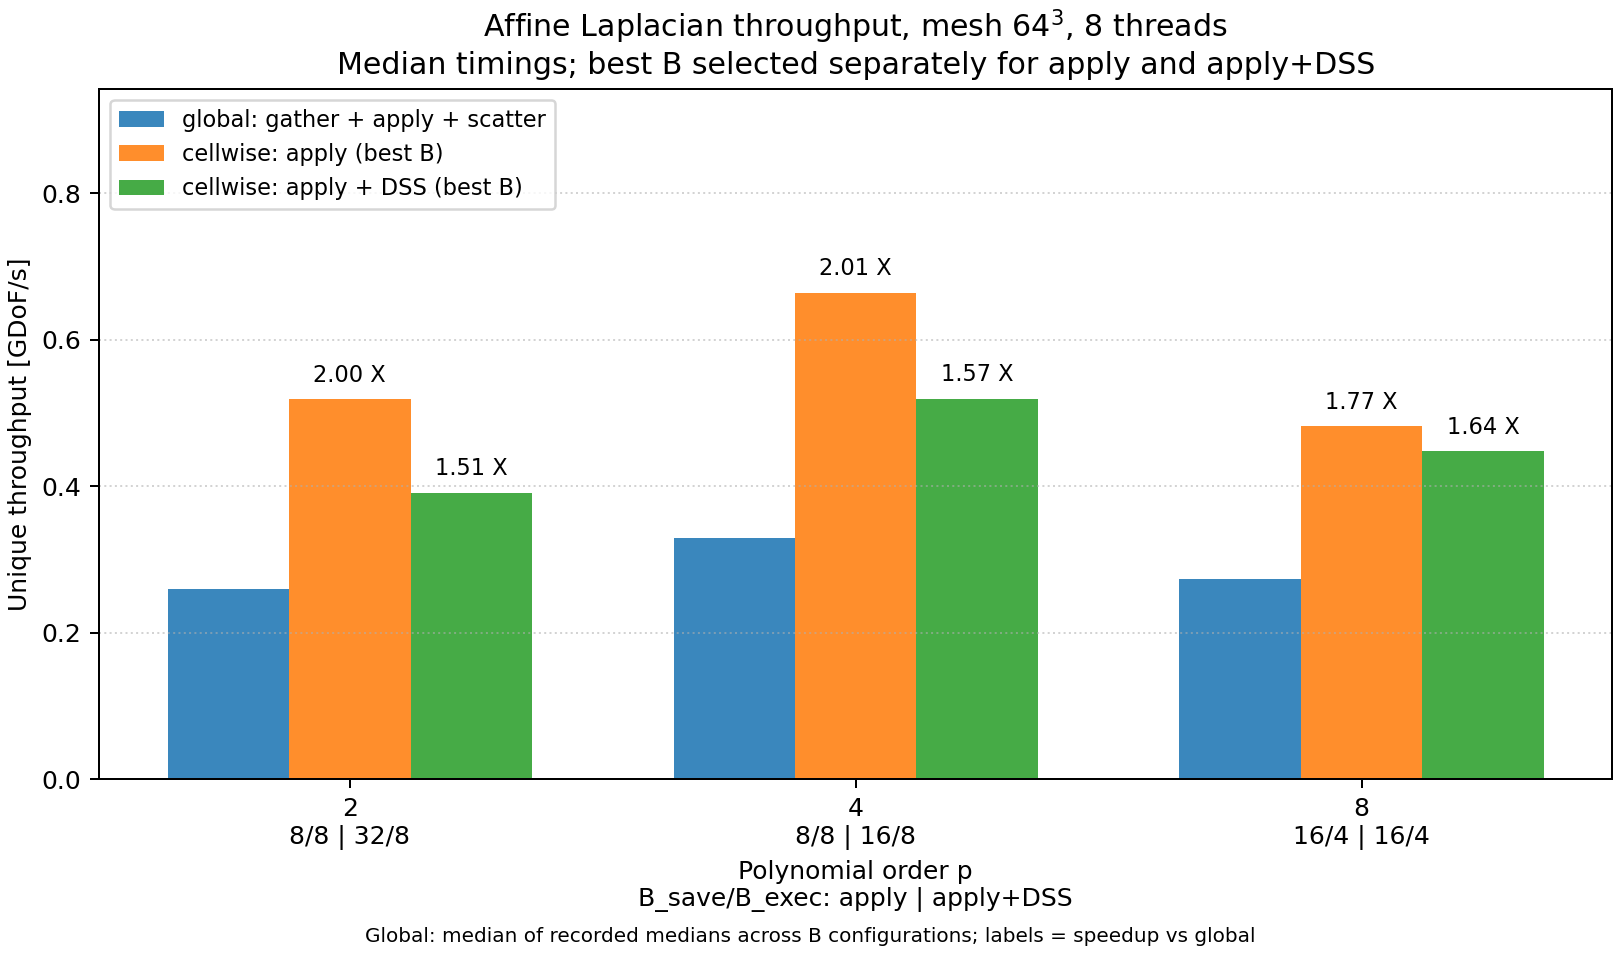
\includegraphics[width=0.96\linewidth]{dss_bxyze_affine_laplacian_global_gdof_s_unique_n64_t8_median.png}
 \caption{The same complete-operator comparison on the \(64^3\)-element
 macro mesh, with one thread (top) and eight threads (bottom). Labels above
 orange and green bars give speedups against the common global baseline.}
 \label{fig:affine-throughput-64}
\end{figure}

Table~\ref{tab:affine-best} records the choices and values used in these plots.
For example, at \(p=4\) on \(64^3\) elements with eight threads, cell-wise
apply reaches \(0.664\) GDoF/s and apply+DSS reaches \(0.519\) GDoF/s,
against \(0.330\) GDoF/s for the global baseline. The selected execution
batch is eight elements there, but four elements at \(p=8\).

\begin{table}[htbp]
 \centering\small
 \setlength{\tabcolsep}{3.5pt}
 \begin{tabular}{rrrrrrrrrr}
 \toprule
 $n$ & Threads & $p$ & $B_s/B_e$ A & $B_s/B_e$ D
 & $\mathcal T_G$ & $\mathcal T_A$ & $\mathcal T_D$
 & $\sigma_A$ & $\sigma_D$\\
 \midrule
 16 & 1 & 2 & 16/4 & 16/4 & 0.060 & 0.100 & 0.093 & 1.68 & 1.55\\
 16 & 1 & 4 & 16/8 & 16/8 & 0.069 & 0.101 & 0.097 & 1.47 & 1.41\\
 16 & 1 & 8 & 4/4 & 16/4 & 0.048 & 0.076 & 0.072 & 1.59 & 1.50\\
 16 & 8 & 2 & 64/8 & 16/16 & 0.207 & 0.309 & 0.167 & 1.49 & 0.80\\
 16 & 8 & 4 & 16/8 & 16/8 & 0.369 & 0.630 & 0.474 & 1.71 & 1.29\\
 16 & 8 & 8 & 8/4 & 8/4 & 0.331 & 0.554 & 0.514 & 1.67 & 1.55\\
 \midrule
 64 & 1 & 2 & 4/4 & 32/4 & 0.048 & 0.089 & 0.068 & 1.88 & 1.42\\
 64 & 1 & 4 & 8/8 & 16/8 & 0.057 & 0.097 & 0.079 & 1.71 & 1.39\\
 64 & 1 & 8 & 4/4 & 16/4 & 0.042 & 0.075 & 0.068 & 1.78 & 1.63\\
 64 & 8 & 2 & 8/8 & 32/8 & 0.259 & 0.519 & 0.391 & 2.00 & 1.51\\
 64 & 8 & 4 & 8/8 & 16/8 & 0.330 & 0.664 & 0.519 & 2.01 & 1.57\\
 64 & 8 & 8 & 16/4 & 16/4 & 0.273 & 0.482 & 0.448 & 1.77 & 1.64\\
 \bottomrule
 \end{tabular}
 \caption{Selected configurations for complete-operator median timings.
 \(n\) is the macro-element count per axis. G denotes the global baseline,
 A cell-wise apply and D cell-wise apply+DSS. Throughputs are in GDoF/s.
 Both speedups use the median-of-medians global baseline of the plots.}
 \label{tab:affine-best}
\end{table}

\FloatBarrier
\subsection{Interpretation and next steps}

The complete operator adds metric application, transpose contractions and
nodal output to the gradient component. Those stages have different memory
access patterns and working sets, so the gradient speedup alone does not
predict the complete-operator speedup. The component benchmark also writes
full-mesh gradients, whereas the complete kernel consumes them batch by batch.
The two benchmarks therefore measure different work and retain different
outputs.

DSS adds interface traffic and synchronization to the cell-wise path.
On the \(16^3\) mesh at \(p=2\) with eight threads, apply alone is faster
than the global baseline, but apply+DSS is slower
(\(\sigma_A=1.49\), \(\sigma_D=0.80\)).
On \(64^3\), the selected apply+DSS configurations are faster in all measured
orders and thread counts. This supports including DSS in block tuning:
the best apply configuration need not minimize the total time.
Differences between two independently selected minima should not be treated
as a direct measurement of DSS cost at one fixed block configuration.

The results identify useful block choices for this machine and protocol;
they do not establish a universal optimum or a hardware bandwidth limit.
Cache state, register allocation, working-set size and thread scheduling
can all affect the timings. SIMD instructions and hardware counters would
be needed to attribute a particular slowdown to a specific resource.
Selection uses the same measurements displayed in the plots, so independent
runs with fixed selected blocks remain useful to assess repeatability.
The two mesh sizes also use different repetition counts.

The first proposed kernel optimization is the metric/weight fusion into
forward z evaluation described above. Further work includes padded final
blocks and DSS for general hexahedral adjacency. The full solver cost would
also include its vector operations, reductions and any representation
conversions. Current timings assume persistent BXYZE input; a workflow
converting from global storage on every apply must include that conversion.

\subsection{Files and reproduction}

The complete implementation and measurements are in:
\begin{itemize}
 \item Public prepared-operator interface and main implementation:\\
 {\small\path{operators/dss/sfem_dss_bxyze_affine_laplacian.hpp}} and\\
 {\small\path{operators/dss/sfem_dss_bxyze_affine_laplacian.cpp}}.
 \item Forward, metric and transpose helpers:\\
 {\small\path{operators/dss/sfem_dss_bxyze_affine_laplacian_inline.hpp}}.
 \item Geometry setup:\\
 {\small\path{operators/dss/sfem_dss_bxyze_geometry.cpp}}.
 \item Structured assembly:\\
 {\small\path{operators/dss/sfem_dss_bxyze_structured.cpp}}.
 \item Complete-operator benchmark:\\
 {\small\path{frontend/ops/dss/benchmark/sfem_DSSBXYZEAffineLaplacianGlobalBench.cpp}}.
 \item Full 300-row CSV and 24-row independent-optima summary:\\
 {\small\path{frontend/ops/dss/benchmark/dss_bxyze_affine_laplacian_global_bench.csv}} and\\
 {\small\path{frontend/ops/dss/benchmark/dss_bxyze_affine_laplacian_global_bench_best.csv}}.
 \item Throughput plotting script:\\
 {\small\path{frontend/ops/dss/benchmark/plot_dss_bxyze_affine_laplacian_global.py}}.
\end{itemize}

From the repository root, using a Release build targeting the M4 Pro with
OpenMP enabled, the default sweep and plots can be reproduced with:
\begin{lstlisting}[language=bash]
PYTHONPATH=python OMPI_MCA_btl=self OMP_NUM_THREADS=8 \
    build/sfem_DSSBXYZEAffineLaplacianGlobalBench

PYTHONPATH=python /path/to/venv/bin/python \
    frontend/ops/dss/benchmark/plot_dss_bxyze_affine_laplacian_global.py
\end{lstlisting}
The per-mesh repetition defaults are described above. Explicit
\texttt{--repeat} and \texttt{--warmup} options override them.
The benchmark also accepts degree, mesh-size, thread-count and block-size
filters, and an \texttt{--output} CSV path. Its output files are overwritten
on a new invocation, so a partial rerun should use a separate output path.
The plot script requires Matplotlib and accepts \texttt{--size 64},
\texttt{--threads 8} and \texttt{--statistic best} filters; the figures here
use the default median statistic. It generates throughput plots only.

\begin{thebibliography}{9}
 \bibitem{KronbichlerKormann2019}
 M.~Kronbichler and K.~Kormann,
 \emph{Fast matrix-free evaluation of discontinuous Galerkin finite element
 operators}, ACM Transactions on Mathematical Software, 45(3), Article 29, 2019.
 \href{https://doi.org/10.1145/3325864}{doi:10.1145/3325864}.

 \bibitem{dealIIEvaluationKernels}
 deal.II contributors,
 \href{https://dealii.org/developer/doxygen/deal.II/evaluation__kernels_8h_source.html}
 {\emph{Matrix-free evaluation kernels}, online source documentation}.
\end{thebibliography}

\end{document}
